\chapter{Proposed Method}
\label{chap-method}
In this chapter, we present our solution for tackle the interactive volume object segmentation. Our proposed approach include reference and propagation module. At first, the pipeline of the method is shown. Then, each module is introduced and the detailed implementation is presented. We apply the distillation technique not only in architecture design but also in the training strategy stage. Finally we dive deep in the potential of loss function especially for medical.

\section{Overview}
\label{sec:overview}

\subsection{A brief introduction to Information Retrieval and the merits of Video-Text Retrieval}
%  paragraph 1
In recent years, we are witnessing impressive growth in both computer hardware and software, which have contributed to the outcomes’ improvement of many expensive tasks, including search.
Information Retrieval (IR), or search in common, is a long-history task claimed to appear in the third century BC in an early type relevant to library administration \cite{eliot2009companion}.
What people know of this terminology today is usually related to electronic devices and the Internet. For example, we may seek a friend’s name in a phonebook or look for a song from its lyrics, a movie from its content by using some search engines.
When we do not know something, instead of going to the library or any kind of information center like we did in the past, most of us constantly “google” it at first.
All of those examples, in fact, are associated with something called Information Retrieval System (IRS) - the implementation of any specific IR theory into the computer operation.
An IR system feeds a query in a particular type as input and gives back the most relevant results to the user through automatic matching methods between the input and data sources (see figure \ref{fig:IR_structure}).
\begin{figure}[!t]
    \centering
    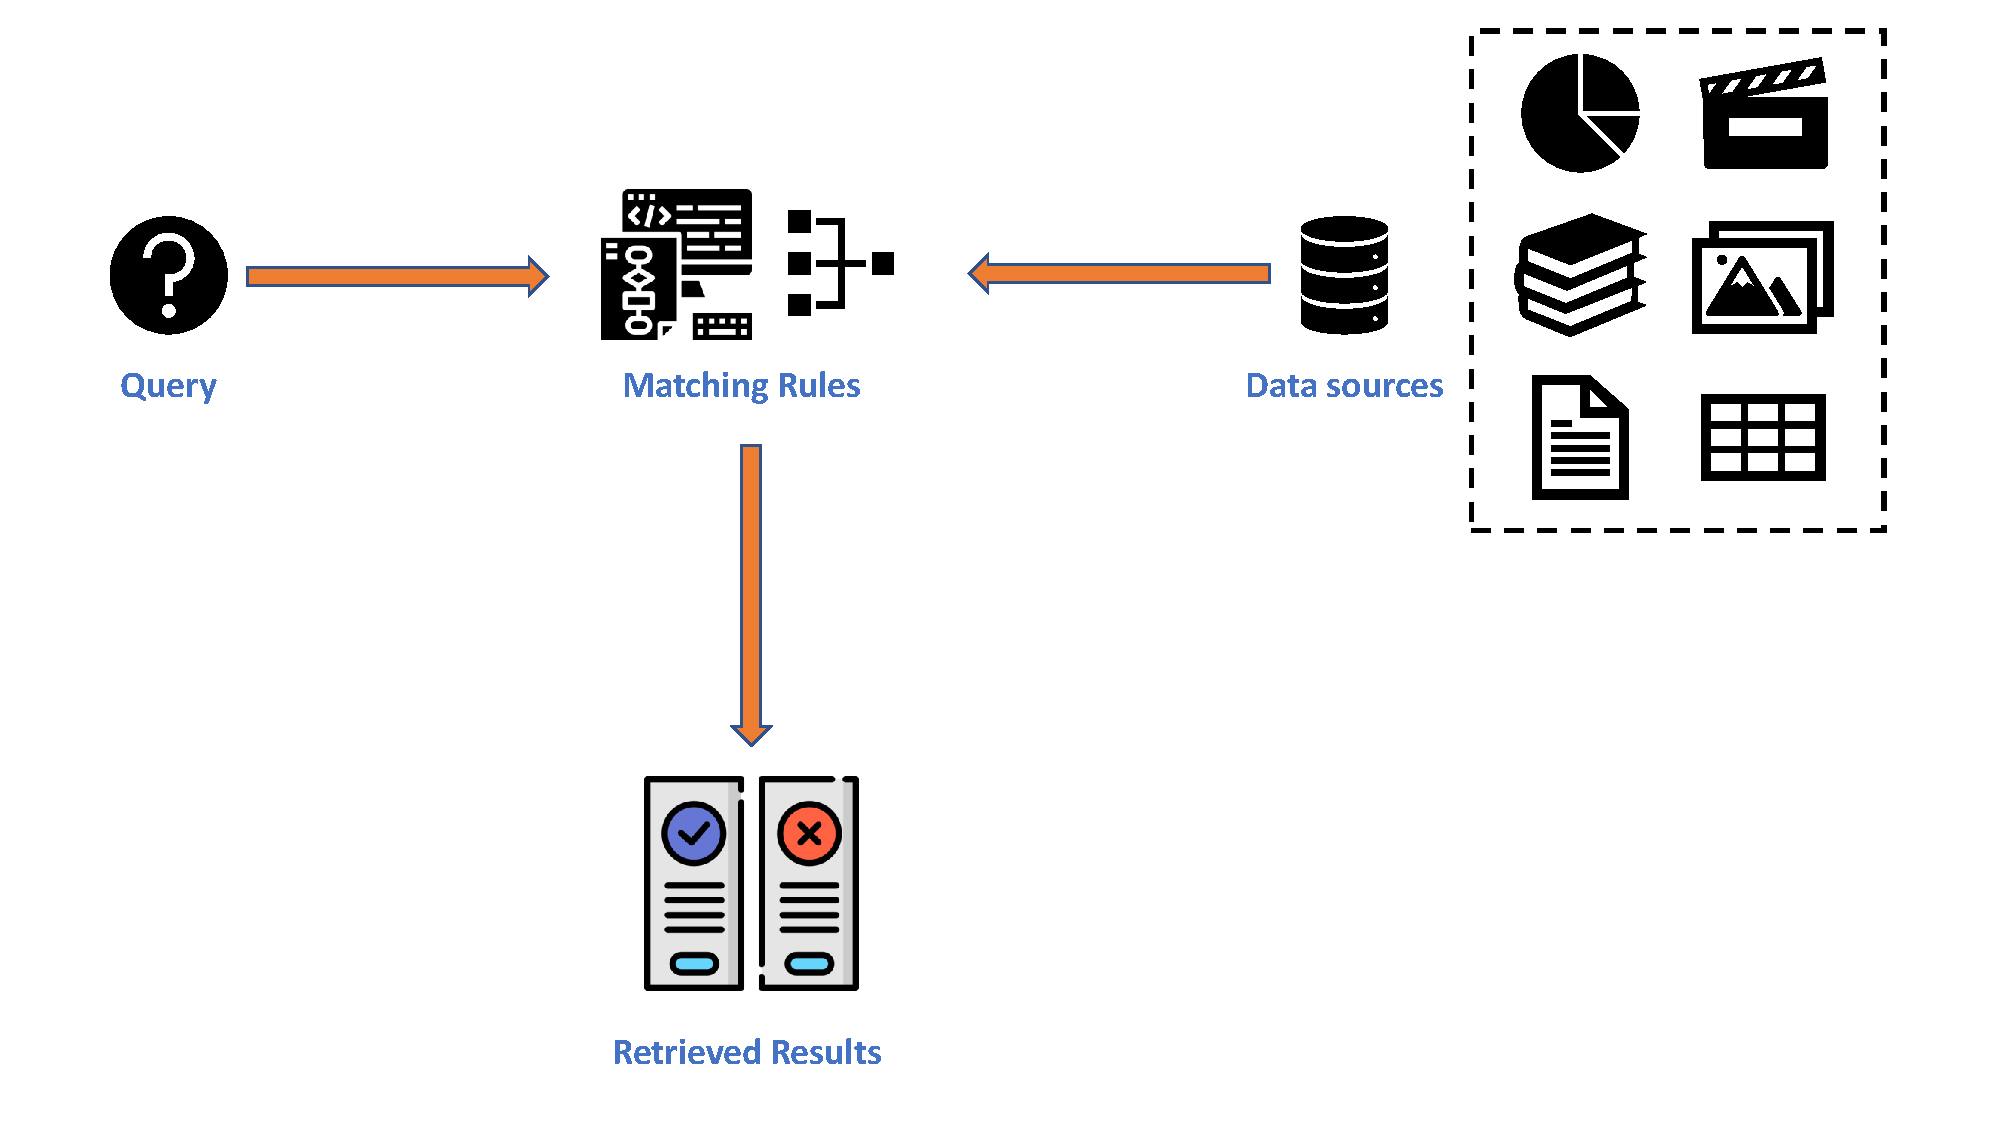
\includegraphics[width=\linewidth]{resources/images/overview/IR_structure.pdf}
    \caption{A simple overview of the Information Retrieval System}
    \label{fig:IR_structure}
\end{figure}
The need for such things occurred due to the increasingly rapid rise in data size and various kinds of information in different areas (like multimedia, website, scientific publication, etc.), making traditional searching techniques no longer cope.
In any IRS, there are always two aspects to deal with: system operation and matching algorithms. Since the first application in the 1940s, it has been developed continuously until now, with many essential milestones \cite{sanderson2012history} tackling both aspects.

%  paragraph 2
As the computing environment changes from time to time, many applications of IR have been suggested, like search on social networks, desktop element search, or one research hotspot recently named cross-modal retrieval.
This task aims to pick out relevant data across different modalities, such as image-text, video-text, audio-text.
Maragos et al. \cite{maragos2008multimodal} stated two future challenges with multimodal applications, including (i) Natural access and high-level interaction with multimedia databases and (ii) Detecting, recognizing and interpreting objects, events and human behavior in multimedia videos by processing combined audio-video-text data.
This statement also reflects two aspects that people always deal with the IRS, as mentioned above.
In research, people may care more about the method aspect than the other.
Traditional methods with manually designed representations, features and matching functions lack the ability to tackle complex IR tasks like multimodal interaction when those tasks require a deeper understanding of document contents and the user information needed \cite{culpepper2018research}.
However, thanks to an ever-stronger influence of Deep Learning \cite{goodfellow2016deep,lecun2015deep} in the 2010s decade, many problems raised in this field have resulted in better performance, letting people expect a new generation of robust and intelligent cross-modal Information Retrieval Systems.

%  paragraph 3
Also, humans have recently witnessed a rapid explosion in the appearance of videos in many aspects of their daily lives.
We all know the potential of videos in entertainment, communication, data analysis, etc.
The rise of video-based online services like YouTube, Netflix, along with the traditional TV program, has inspired Computer Vision (CV) experts to pay more attention to this resource. Additionally, natural language (NL) is one of the most effective means to describe those video contents.
From this point of view, the task of searching videos via text queries, or video-text retrieval, in short, becomes a desirable function in intelligent systems.
This problem takes (a) natural language text description(s) as input and outputs a sorted list of videos in terms of semantic relevance.
A lot of neuron network-based methods, focusing on transforming text input and video’s particular contents into the same subspace and measuring their similarity, have worked efficiently.
However, each video retrieval task has its own specificities among the diversity of the visual world, besides some in-tackling challenges like the semantic gap between two modalities, lack of annotated video-caption, or complicated consideration of temporal information, making no universal utilization approach fit for all such retrieval problems.
Therefore, caption-to-video retrieval is still attracting researchers to resolve in different areas.

\subsection{A brief introduction to Intelligent Transportation/Traffic System and the merits of Vehicle-oriented Computer Vision Tasks}
%  paragraph 1
Transportation is a non-separable part of any country, playing an essential role in different aspects of our daily life.
Residents, governments, and businesses almost depend on it to access resources.
Therefore, the advent of Intelligent Transportation/Traffic System (ITS), a significant factor contributing to the concept of smart city and to the development of modern civilization, is inevitable.
The implementation of ITS is widely accepted and used in many countries today when the governments recognize (i) the rapid growth of the human population, (ii) high-speed urbanization, and (iii) increasing vehicle ownership.
Though there are multiple modes of transportation, the roadway is the most common route.
So this kind of system aims to address a wide range of road traffic issues via advanced technologies, solving at three main levels: society, the road administrator, and drivers.
By providing different modules centering around the people-vehicle-road relation, and other traffic objects, it helps improve the safety, efficiency,  and environmental friendliness of the transportation.

%  paragraph 2
In an ITS that inherits Deep Learning works, Fan et al. \cite{fan2020deep} have shown that there are four major services in the architecture, as illustrated in figure \ref{fig:ITS_structure}.
\begin{figure}[!t]
    \centering
    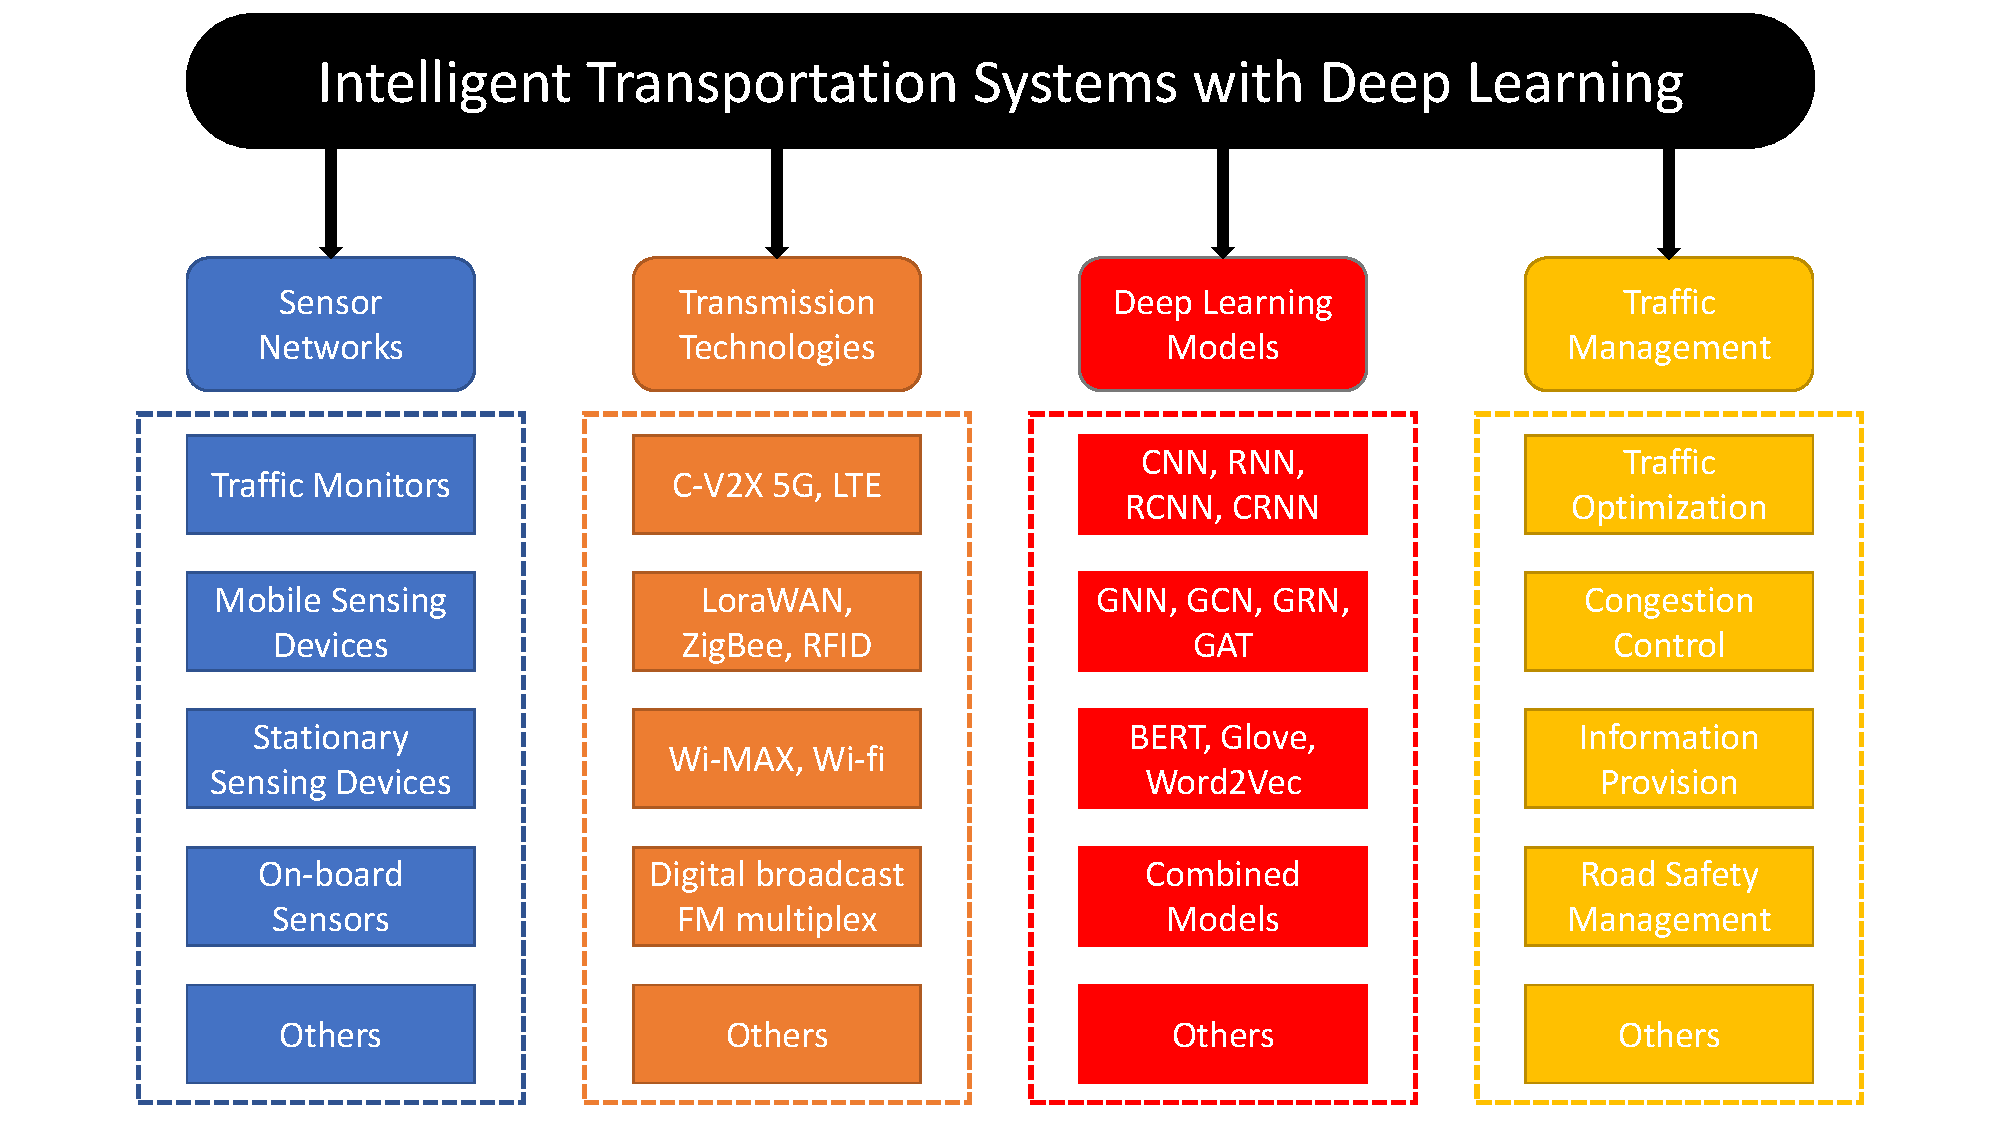
\includegraphics[width=\linewidth]{resources/images/overview/ITS_structure.pdf}
    \caption{Major components of a Deep Learning-based Intelligent Transportation/Traffic System.}
    \label{fig:ITS_structure}
\end{figure}
The Sensor Networks service is in charge of collecting real-time data then sends it through the Transmission Technologies service.
By exploiting the data, the Deep Learning Models service is responsible for building models that can perform well in particular tasks before integrating them into practical modules of the Traffic Management service.
When it comes to Computer Vision applications in such systems, many problems are mainly related to vehicles.
This is because transportation is vehicle-centered, unlike other areas, which are often people-focused.
Thanks to the widespread installment of 24/7 surveillance cameras on roads and highways, people can obtain massive traffic data.
Although the potential for video analytics from that data is enormous to be leveraged, it has not been exploited optimally.
Some tasks have received high-accurate state-of-the-art results, such as Vehicle Counting \cite{lu2021robust, dai2019video, asha2018vehicle} or Vehicle Reidentification \cite{luo2021empirical, Khorramshahi_2019_ICCV, zhu2019vehicle}, but some are still far from saturated outcomes.
Two major hurdles include the insufficiency of labels and the lack of high-performance models capable of converting data into valuable insights.
Regarding the model, since the vehicle is a particular domain and non-human, many pre-trained models cannot be applied directly to this object.
Therefore, CV researchers in this field still face so many significant challenges.
And, there should be something that can attract attention to address such issues.

%  paragraph 3
For those reasons, in parallel with the works of individuals, there are also organizations holding vehicle-oriented contests in order to find solutions from talented candidates.
Not stopping there, through these contests, people hope for deployments of submitted models into a realistic environment. 
One of the hottest contests is the AI City Challenge \cite{Naphade17AIC17, Naphade18AIC18, Naphade19AIC19, Naphade20AIC20, Naphade21AIC21}, opening continuously since 2017.
This contest primarily focuses on accurate, robust, and efficient approaches, so the organizers provide relatively sufficient labeled datasets \cite{Feng21CityFlowNL, Tang19CityFlow, Yao20VehicleX} as well as the evaluation system.
Their problems range from the mentioned tasks above to others like Velocity Estimation, Anomaly Detection, Vehicle Tracking, etc., whose insights may be inspired by various techniques.
In the latest edition, the 5th AI City Challenge \cite{Naphade21AIC21} has proposed a novel advanced track named Natural Language-Based Vehicle Retrieval (NL-based VR), which needs an effective combination of subtasks including motion detection, appearance recognition and content-based video retrieval.
There are still other tasks from other competitions, but finally, they all have the same goal: to solve real-world traffic issues and implement them into the Intelligent Transportation/Traffic System.
\section{Preprocessing}
\label{sec:preprocess}
For preprocessing, we apply Windowing technique  \cite{windowingct17yahya} with different levels and widths to target specific parts of human organs. Windowing, also known as grey-level mapping, contrast stretching, histogram modification or contrast enhancement is the process in which the CT image grayscale component of an image is manipulated via the CT numbers; doing this will change the appearance of the picture to highlight particular structures. The brightness of the image is adjusted via the window level, window level determines the central or midpoint grey value for the range of HU displayed in the image. Ideal imaging of different tissues depends on the window level. The contrast is adjusted via the window width. A wide window (400-2000 HU) is suitable for examining structures of vastly different attenuation values. For instance, chest structures are best viewed using a wide window.

In or experiments, we apply 3 wide windows corresponding with 3 different versions of a single slice by highlight the abdomen, chest, and spine groups and stack it to one as a three-channel image (Fig. \ref{fig:windowingct}). The window parameters in our experiments are shown in table \ref{table:window_params}
\begin{table}[]
\centering
\caption{Window parameters}\label{table:window_params}
\begin{tabular}{| l | c c |}
\hline
Group      & Window level & Window width \\ \hline
Spine-bone & 900          & 1400         \\ \hline
Tissues    & 200          & 350          \\ \hline
Chest      & 787          & 2137         \\ \hline
\end{tabular}
\end{table}

Where the group of the soft tissue masses can be determined by merging of the abdomen soft tissues and liver. The chest group, which consists of the lungs and mediastinum. By re-calculating the window information from the min value and max value of selected range, these window parameters can be accurately determined.

\begin{figure}[!h]
    \centering
    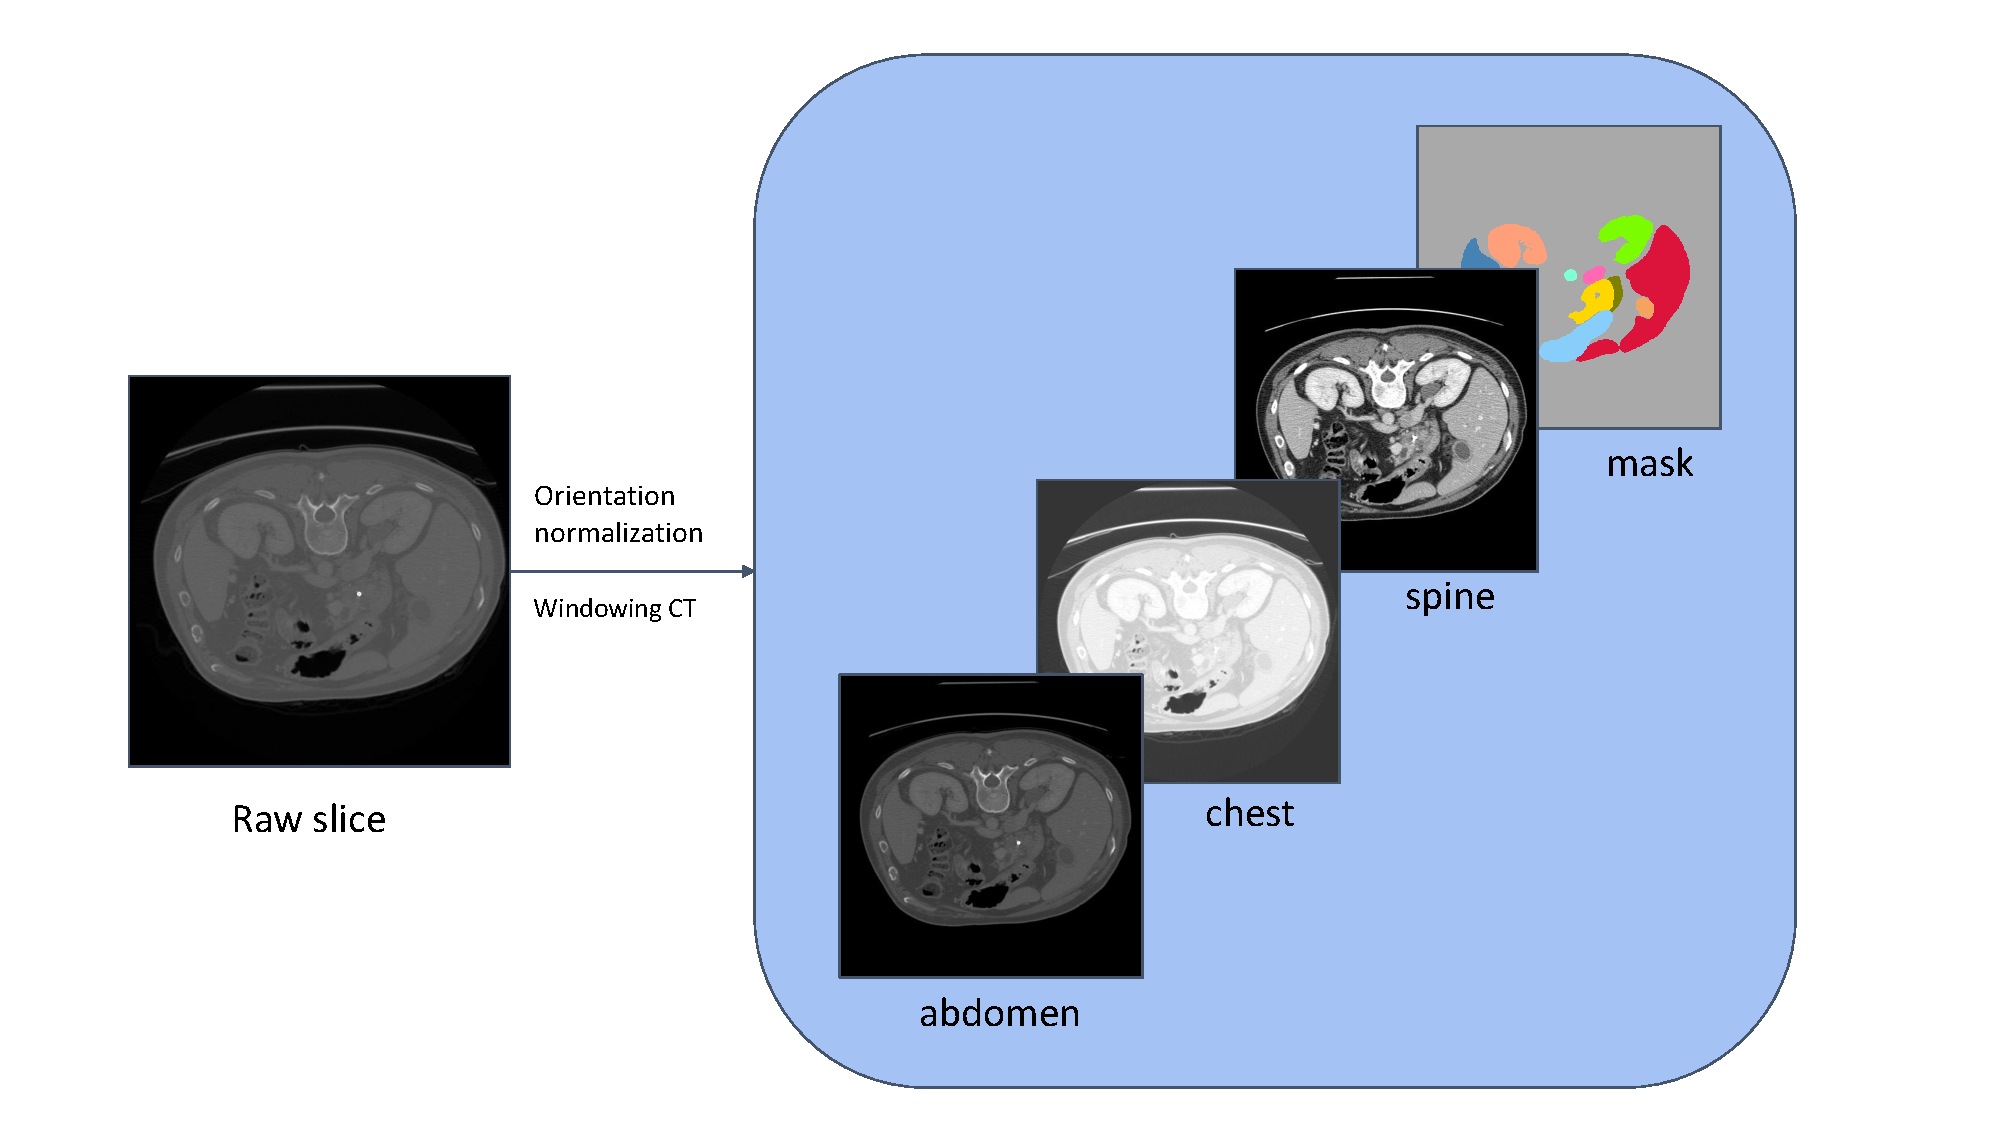
\includegraphics[width=\textwidth]{resources/new_images/preproc.pdf}
    \caption{Windowing CT. 3 different versions are generated from an original slice. }
    \label{fig:windowingct}
\end{figure}

In addition, we choose the axial plane to cut the slices from the CT volumes since this plane has various dimension sizes. 
Due to some relatively small organs, it might be better to keep the original size of the slices without any cropping, resampling, or resizing methods.
The image is rotated to a predefined angle, then divided by 255 for normalization before going through the next step.
\pagebreak
\section{Reference module}
\label{sec:reference}
\begin{figure}[!htb]
    \centering
    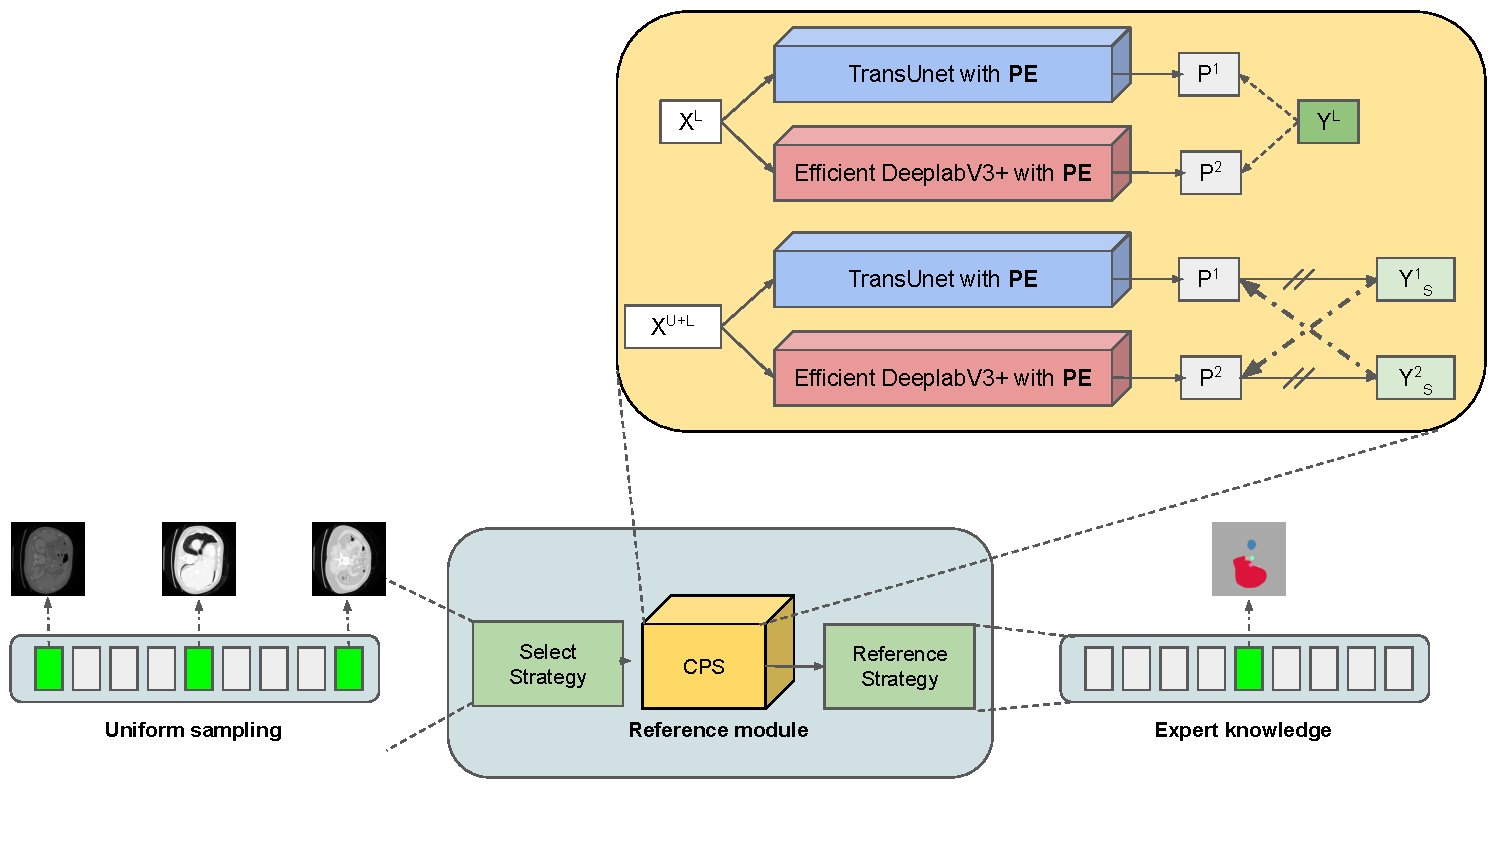
\includegraphics[width=\textwidth]{content/resources/new_images/reference.pdf}
    \caption{The reference module. The semi-supervised technique CPS is applied in both training and inference stage to enhance the precision of model prediction. Strategies are used to smartly choose slices that are informative for the next stage. }
    \label{fig:reference}
\end{figure}


This module is expected to provide a suggestion of a minimal amount of slices and predicted masks that might contain the most information describing the entire CT Volume. Fig \ref{fig:reference} describes the details of this module.

To utilize the enormous number of unlabeled data, we apply the recent semi-supervised method that performs effectively on several other datasets, which is called Cross Pseudo Supervision (CPS) \cite{cps21chen} (yellow cube in Fig. \ref{fig:reference}).
CPS enables the usage of unlabeled data by following the dual students technique, where two models are trained simultaneously on labeled data while generating pseudo data for their "peer" to learn. In the testing phase, two models predict the same image, and the result is aggregated by summing up.

We adopt two prominent state-of-the-arts 2D segmentation models with highly different learning paradigms for this CPS framework, which is TransUNet \cite{transunet21chen} and DeeplabV3+ \cite{dlv3p18chen}. While DeeplabV3+ traditionally focuses more on the local information, transformers model the long-range relation, so the cross training can help to learn a unified segmenter with these two properties at the same time. In short, we choose TransUNet and DeeplabV3+ due to their ability to compensate each other for better performance. \cite{crosscnntransformer21luo}


% Transformers are a novel architecture that solves sequence to sequence tasks while handling long-range dependencies. Transformers are used standalone or combined with CNN(Convolutional Neural Networks), significantly boosting computer vision tasks

In addition, we also propose a both logical and specialist-based strategy to choose which slices can be further used to boost the performance of the Propagation module. The goal of this action is to preserve only some of the most useful information for the refinement stage.

To elaborate on these strategies, prior to being put into the CPS module for prediction, a small number of slices are uniformly sampled from the processed CT volume. After CPS produces segmentation masks for these slices, another selection step is performed to pick only some of the masks that contain the organs having the largest areas.  
\section{Propagation module}
\label{sec:propagation}
\begin{figure}[!h]
    \centering
    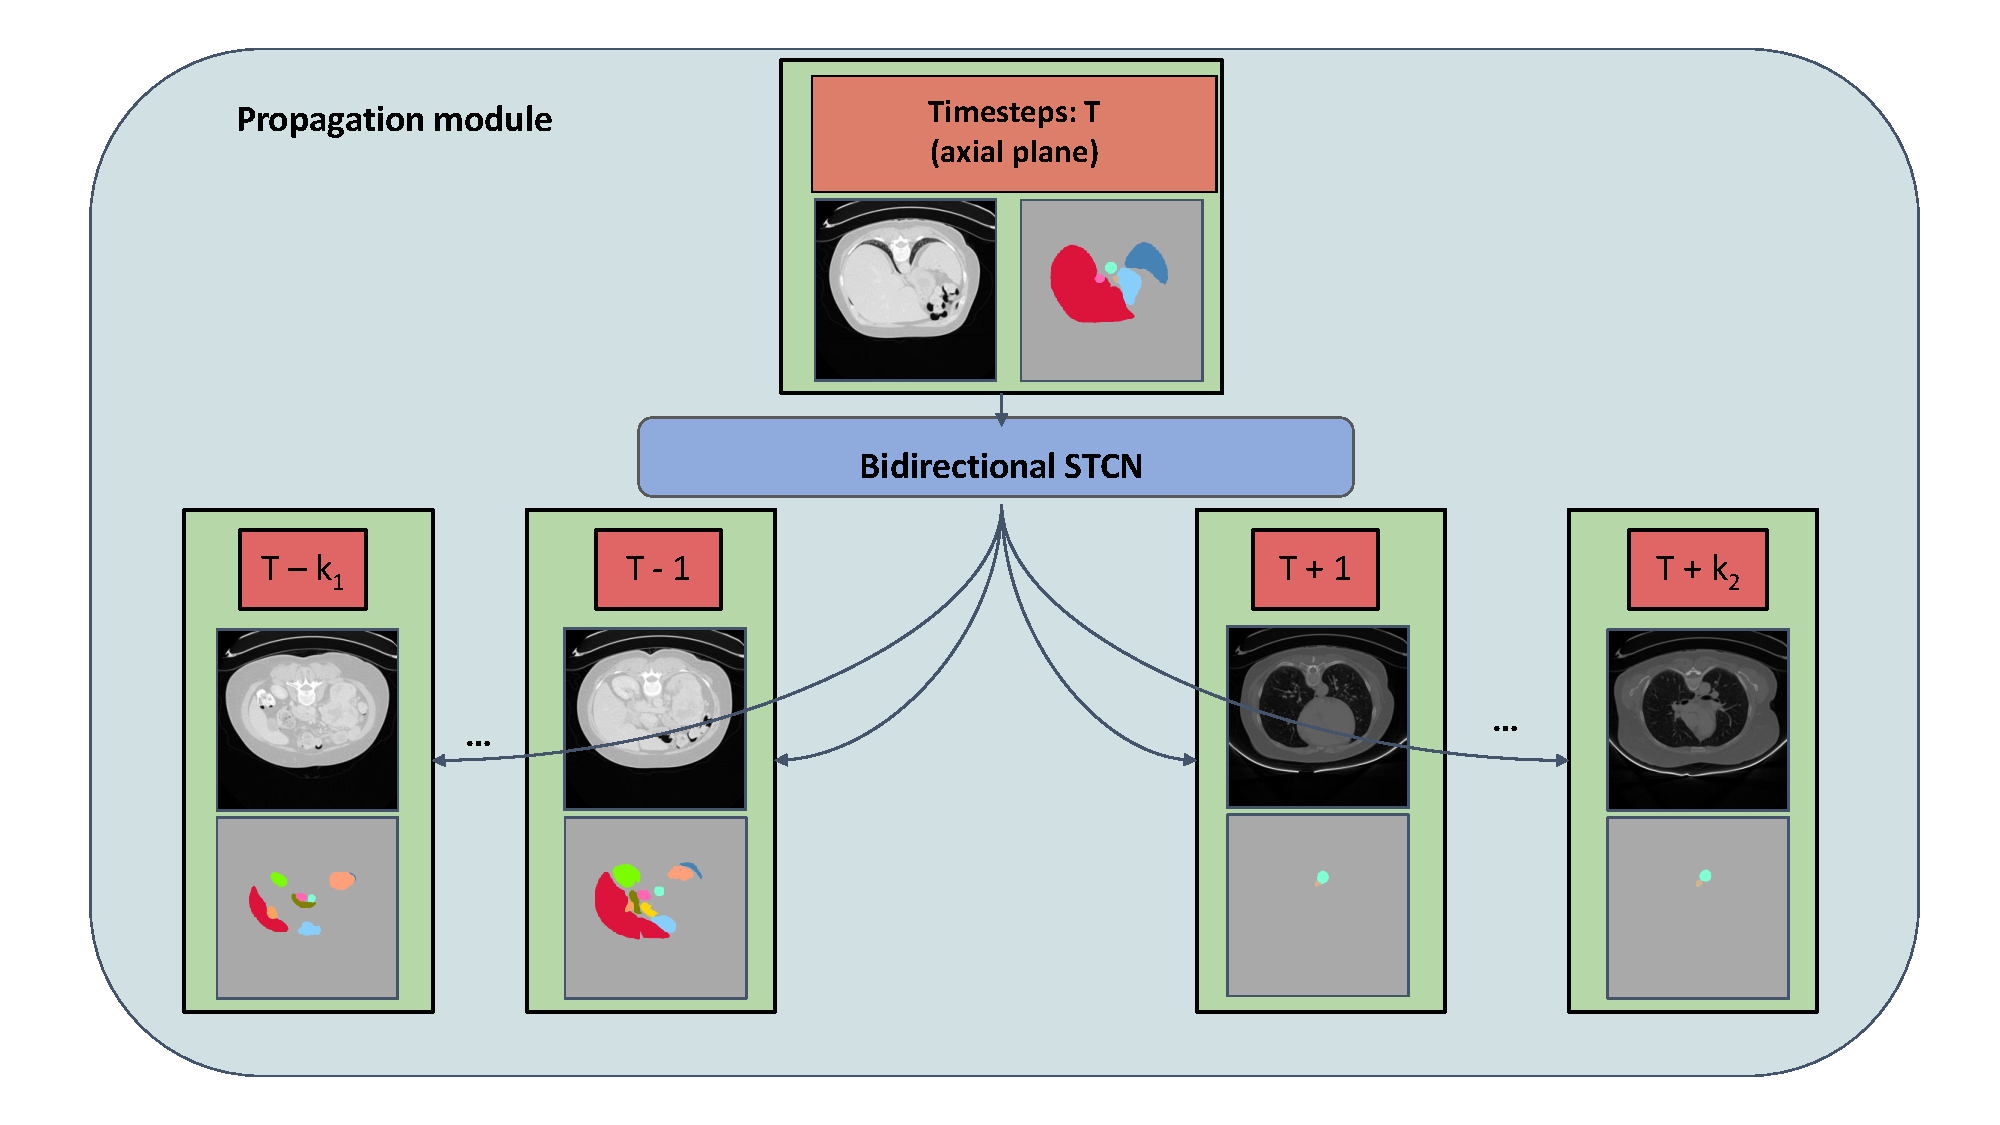
\includegraphics[width=\textwidth]{content/resources/new_images/propagation.pdf}
    \caption{The propagation module. From an annotated slice of CT, at timestep T, STCN can make use of that to spread the information through the entire defined range $[T-k_1, T+k_2]$.}
    \label{fig:propagation}
\end{figure}

This module aims to utilize prior knowledge of given annotated slices from the Reference module to make prediction on the remaining slices, this mechanism can be referred as mask (or label) propagation.

Intuitively, the conventional 2D CNNs cannot comprehend the third dimension information within a CT volume. Thus, in hope of the ability to capture the "temporal" information along the axial plane, we adapt the Space-Time Correspondence Networks (STCN) \cite{stcn21cheng}, which is a semi-supervised segmentation algorithm that has achieved promising results on Video object segmentation problem, to this 3D manner. 

Basically, STCN proposes the use of a memory bank that stores information about previous frames and their corresponding masks and uses them later as prior knowledge. To generate the mask for the current frame, a pairwise affinity matrix is calculated between the query frame and memory frames based on negative squared Euclidean distance, then it is used for supporting the current mask generation \cite{stcn21cheng}. 

Different from the original STCN, we slightly modify it to match the current problem. In the original work, they use only a single dense mask to propagate through the entire video, therefore for the model to perfectly work, that selected mask must contain information about all available classes. For our case to achieve that, we enable the usage of multiple masks for propagation, so that all of these masks should contain enough information about every organs. We also allow the STCN to work in a bidirectional way to enhance the refinement. Fig \ref{fig:propagation} illustrates this process.

Specially, STCN can be simply trained in the binary manner, meaning that each of the abdominal organs can be learned separately. Therefore, the knowledge can be transferred well between different organ classes.
\section{Pseudo Labeling}
\label{sec:labeling}
% \begin{figure}[!htb]
%     \centering
%     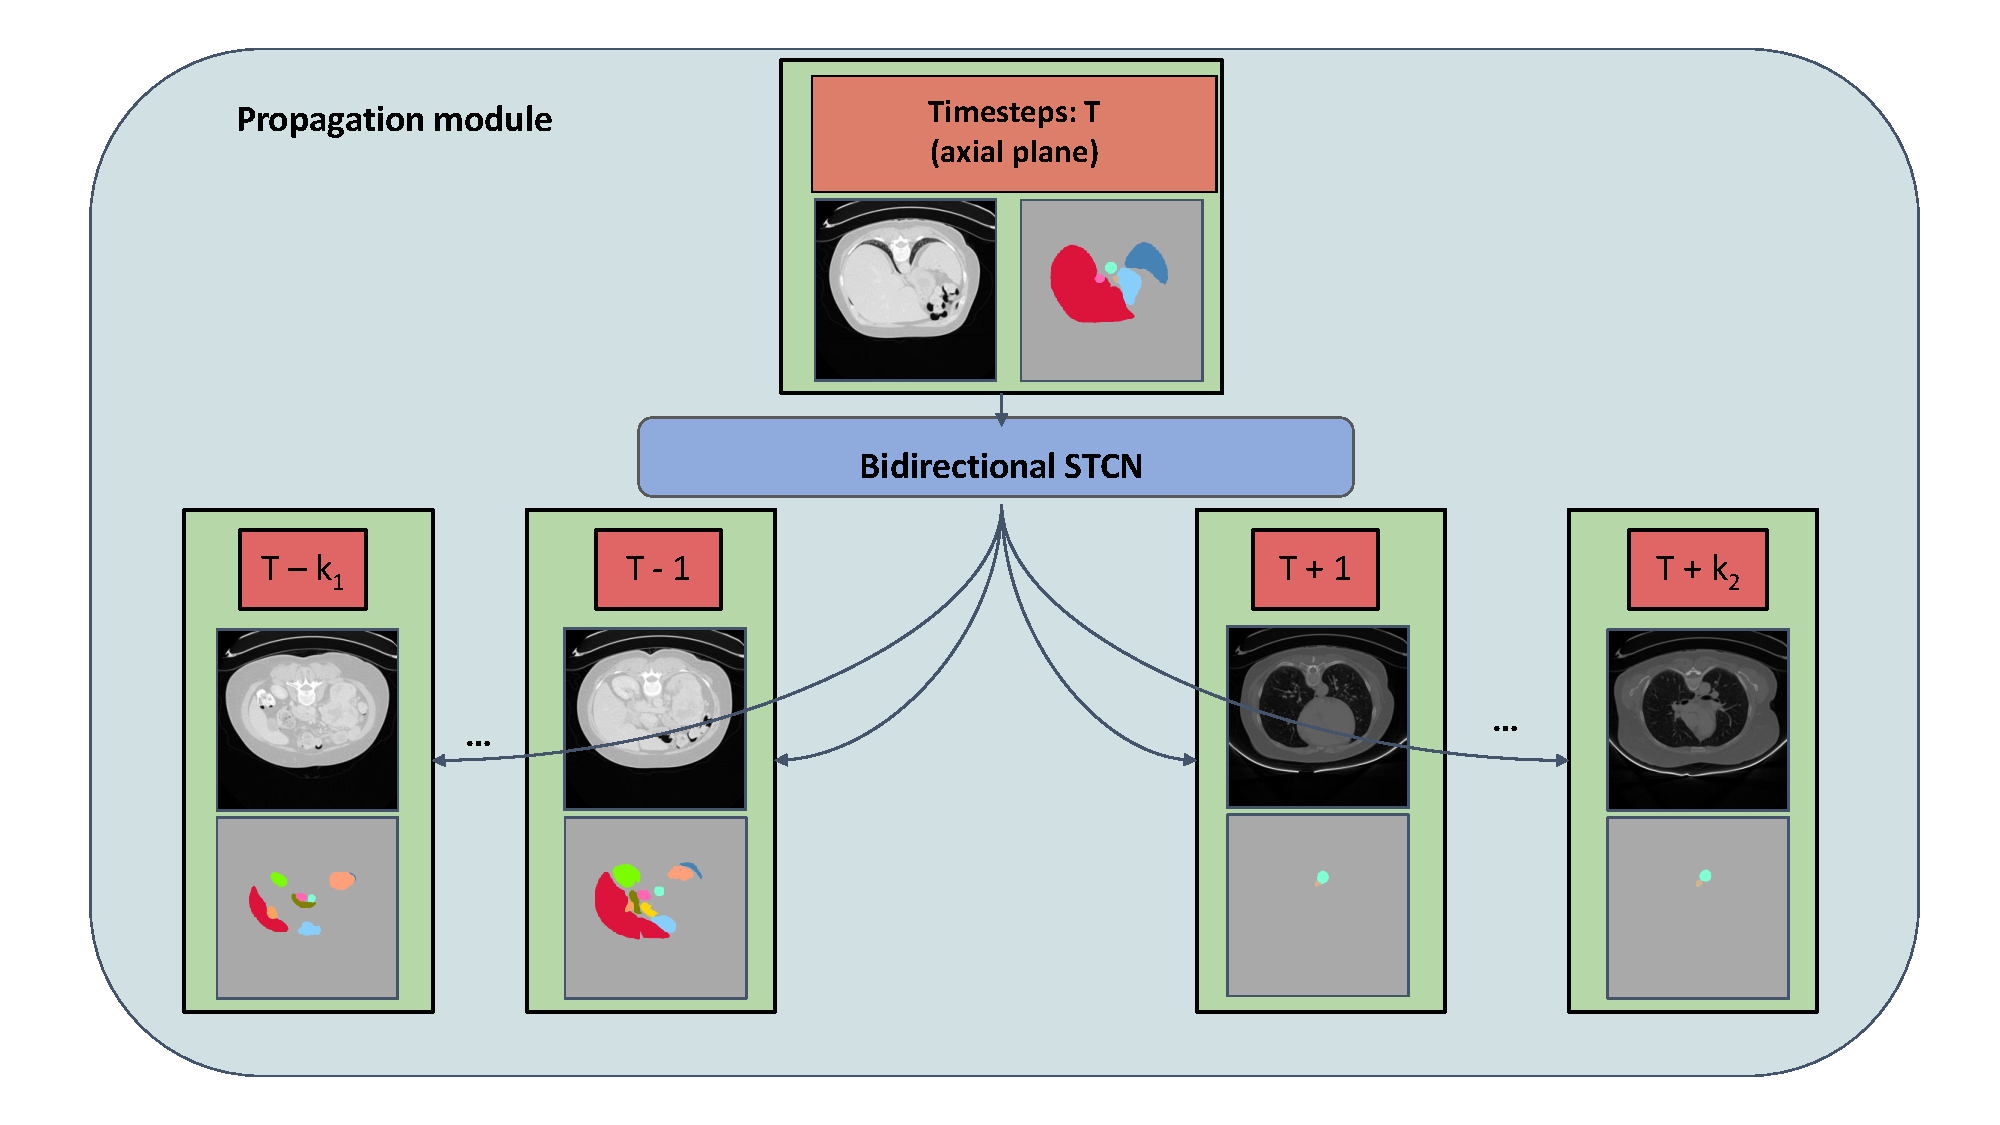
\includegraphics[width=\textwidth]{content/resources/new_images/propagation.pdf}
%     \caption{The propagation module. From an annotated slice of CT, at timestep T, STCN can make use of that to spread the information through the entire defined range $[T-k_1, T+k_2]$.}
%     \label{fig:labeling}
% \end{figure}


Given a vast amount of unlabeled CT volumes, we apply a uncertainty estimation technique to effectively maximize the utilization of the data.

Firstly, several CPS models are trained on the provided labeled data.
Then, we use these trained CPS models to obtain pseudo masks on the unlabeled set. Inspired from \cite{wang2019active}, we calculate the dice scores between these pseudo masks and the aggregated one. The mean of these dice scores will be compared with a threshold to determine whether the aggregated pseudo masks are qualified. Simply speaking, consensus-based assessment is used to evaluate the quality of pseudo labels.

We determine a single score for the $i^{th}$ volume in the unlabeled set as the formulation below:

\begin{align}
        score_{i} &= \frac{1}{K \times M} \sum_{k=1}^{K^{i}} \sum_{m=1}^{M} \text{DSC}(\mathcal{Y}^{k,i}_{m}, \mathcal{Y}^{k,i}_{AVG}) \\
        \text{dsc}  &= \frac{2 |X \cap Y|}{|X| + |Y|}
\end{align}

DSC represents the Dice Score evaluation metric calculating the overlapping area of prediction $X$ and ground truth $Y$. 
Here $\mathcal{Y}^{k,i}_{m}$ indicates the $m^{th}$ model’s output of the $k^{th}$ slice of volume $i$ while $\mathcal{Y}^{k,i}_{AVG}$ is the mask averaged from all $M$ models for the same slice. The easier the sample is, the more inclined the segmentation are to get a similar output if the sample is easier. In contrast, hard samples are more likely to be segmented differently by different models. Hence, we use the proposed score to measure the certainty between models' predictions. Higher score gives more credibility to the prediction, as it is more consistent. 

All aggregated samples that have high certainty are then reused for the next supervised training cycle. And after the training finishes, the same labeling process is repeated until all aforementioned models achieve satisfied performance or every unlabeled data has been used.
\section{Loss functions}
\label{sec:loss}

For the Reference module, we use the prevalent combination of dice loss and cross entropy loss with smoothing value to alleviate the imbalanced number of the small organs, which occurs due to our splitting into slices process. The same settings are used for CPS in its supervised branch whereas only the dice loss is setup for the unsupervised branch. 

For the Propagation module, we implement the online hard example cross entropy (OhemCE or Bootstrapping CE) \cite{ohemce16wu} and also calculate the Lovasz loss \cite{lovasz18berman} at the same time. OhemCE can help reduce the contribution of background label to the final loss. And since STCN is trained on binary task, OhemCE can direct the model to focus on visible difficult objects. Meanwhile, Lovasz loss is commonly used in the past. 


Given y the ground truth mask, and \hat{y} the predicted mask of the model, we reformulate all the losses that we have used in training our networks as below: 

\textbf{Dice loss}

The Dice coefficient is widely used metric in computer vision community to calculate the similarity between two matrices. In recent years, it has also been adapted as loss function known as Dice Loss \cite{sudre2017diceloss}

\begin{align}
        DL (y, \hat{y}) &= 1 - \frac{2\hat{y}y+\epsilon}{\hat{y}+y+\epsilon}
\end{align}

Here, $\epsilon$ is added in both numerator and denominator to ensure that the function is not undefined in edge case scenarios such as when $\hat{y} = y = 0$.

\textbf{Cross-entropy loss}

Cross-entropy is a traditional loss function that is widely used for classification objective, and as segmentation is pixel level classification it works well. It is defined in \cite{yi2004ce} as a measure of the difference between two probability distributions for a given random variable or set of events.
Binary Cross-Entropy is defined as:

\begin{align}
        L_{BCE} (y, \hat{y}) &= -(y log (\hat{y}) + (1-y)log(1-\hat{y}))
\end{align}

\textbf{Online hard example cross-entropy loss}

We et. al \cite{ohemce16wu} propose an online bootstrapping method, which forces networks to focus on hard (and so more valuable) pixels during training. 

Let there be $K$ different categories $c_j$ in a label space. For simplicity, suppose that there is only one image crop per mini-batch, and let there be N pixels $a_i$ to predict in this crop. Let $y_i$ denotes the ground truth label of pixel $a_i$
, and $p_{ij}$ denotes the predicted probability of
pixel $a_i$ belonging to category $c_j$ . Then, the loss function can be defined as

\begin{align}
        L_{OhemCE} &= - \frac{1}{\sum_{i}^{N} \sum_{j}^{K} 1 \{y_i = j \text{ and } p_{ij} < t\}} (\sum_{i}^{N} \sum_{j}^{K} 1 \{y_i = j \text{ and } p_{ij} < t\} log p_{ij})
\end{align}

where t ∈ (0, 1] is a threshold. Here 1{·} equals one when the condition inside holds, and otherwise equals zero. In practice, there should be a reasonable number of pixels kept per mini-batch. Hence, the threshold $t$ will be increased accordingly if the current model performs pretty well on a specific mini-batch.

\textbf{Lovasz-Softmax loss}

 Berman et. al \cite{lovasz18berman} incorporates the softmax operation in the Lovasz extension. Having the similar target as the Dice Loss, The Lovasz extension is a means by which we can achieve direct optimization of the mean intersection-over-union loss in neural networks. In this respect, the Lovasz-Softmax loss can be formulated as follows:
 
 \begin{align}
        L_{lovasz} &= \frac{1}{|C|} \sum_{c \in C} \overline{\Delta_{J_c}} (m(c)) \\
        m_i(c) &= \begin{cases}
                        1 - x_i(c)  & \text{if } c = y_i(c) \\
                        x_i(c)    & \text{otherwise}
                    \end{cases}
\end{align}

where $|C|$ represents the class number, $\Delta_{J_c}$ defines the Lovasz extension of the Jaccard index, $x_i(c) \in [0,1]$ and $y_i (c) \in \{-1,1\}$ hold the predicted probability and ground truth label of pixel $i$ for class $c$, respectively.


% \section{Textual Attribute Extraction}
\label{sec:text_extraction}
\begin{figure}[!htb]
    \centering
    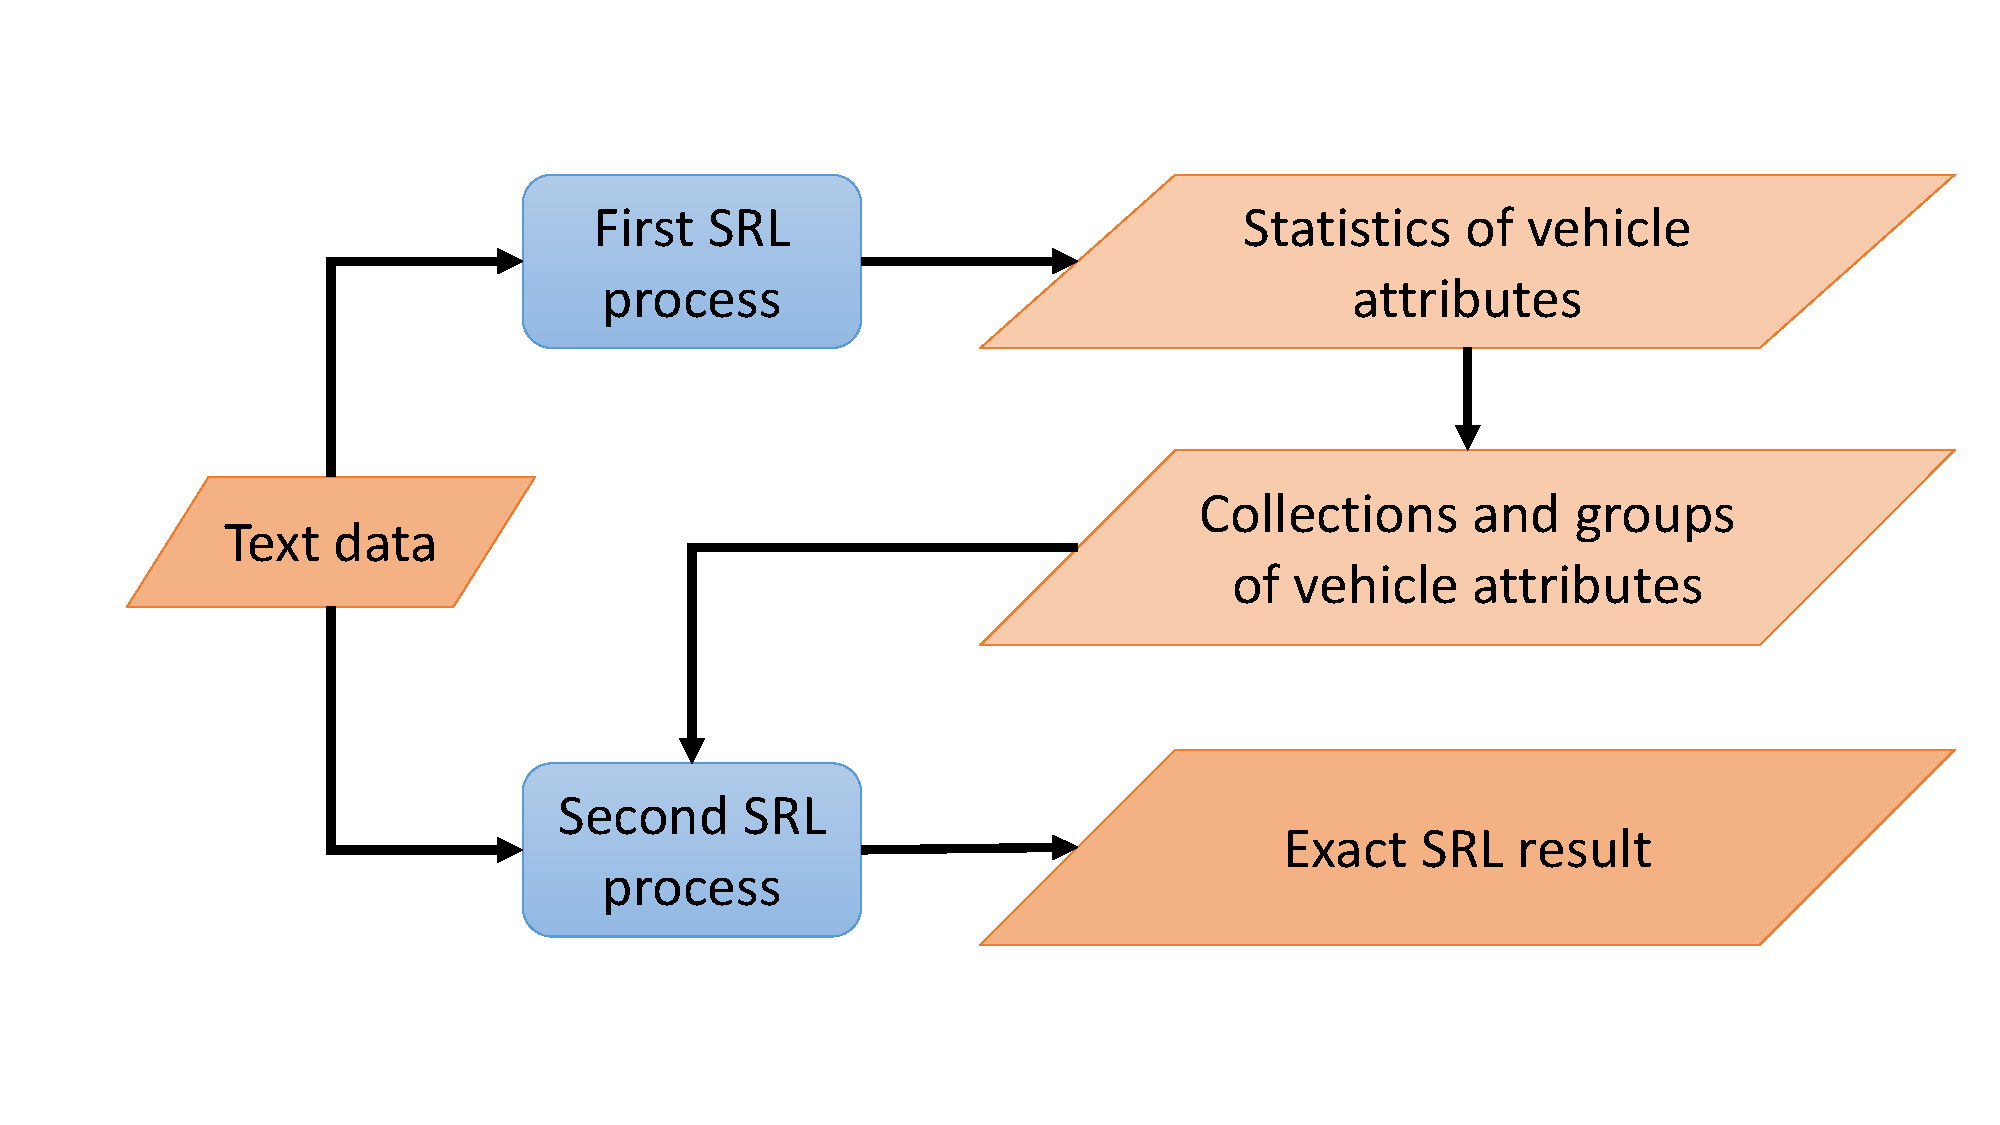
\includegraphics[width=\textwidth]{images/methods/text_branch_overview.pdf}
    \caption{The overview of process flow on text branch.}
    \label{fig:text_branch_overview}
\end{figure}
On such retrieval problems, the text data usually contains rich information about the objects and their activities. Also, this dataset mainly focuses on traffic and vehicle, narrowing the scope of vocabularies but still providing essential information. Therefore, besides feeding the text query into the next-step model, we employ a method to obtain specific query keywords to construct a special collection of vehicle attributes. This task helps us label each query on some categories, useful for later tasks about classification, detector, or re-ranking.
It should be noticed that most of the queries are structured as follow:

\textbf{Vehicle + Action + Optional object(s) + Other information.}

That is the reason we consider English PropBank Semantic Role Labeling (SRL), via the method proposed in \cite{shi2019simple}, as a possibly efficient means to parse verb and noun phrases. A two-phase flow describing the text-branch process is shown in Figure \ref{fig:text_branch_overview}.
\begin{itemize}
    \item First, to analyze the data, we take an SRL extraction on raw data to make statistics on the vehicle's attributes. This process helps us confirm that it is necessary to define potential values about the vehicle types, actions, colors. After filtering the top most frequent and suitable words on each attribute and observing the relation among queries in a track, we create certain groups for three types of the attribute. Figure \ref{fig:group_example} illustrates the result of categorizing.
    \item The second phase of this flow described the heuristic method we build to extract each query on mentioned categories exactly. There are two main stages in this phase, shown in Figure \ref{fig:text_branch_stage_2_overview}.
\end{itemize}

\subsection{Preprocessing stage}
\begin{figure} [!htb]
    \centering
    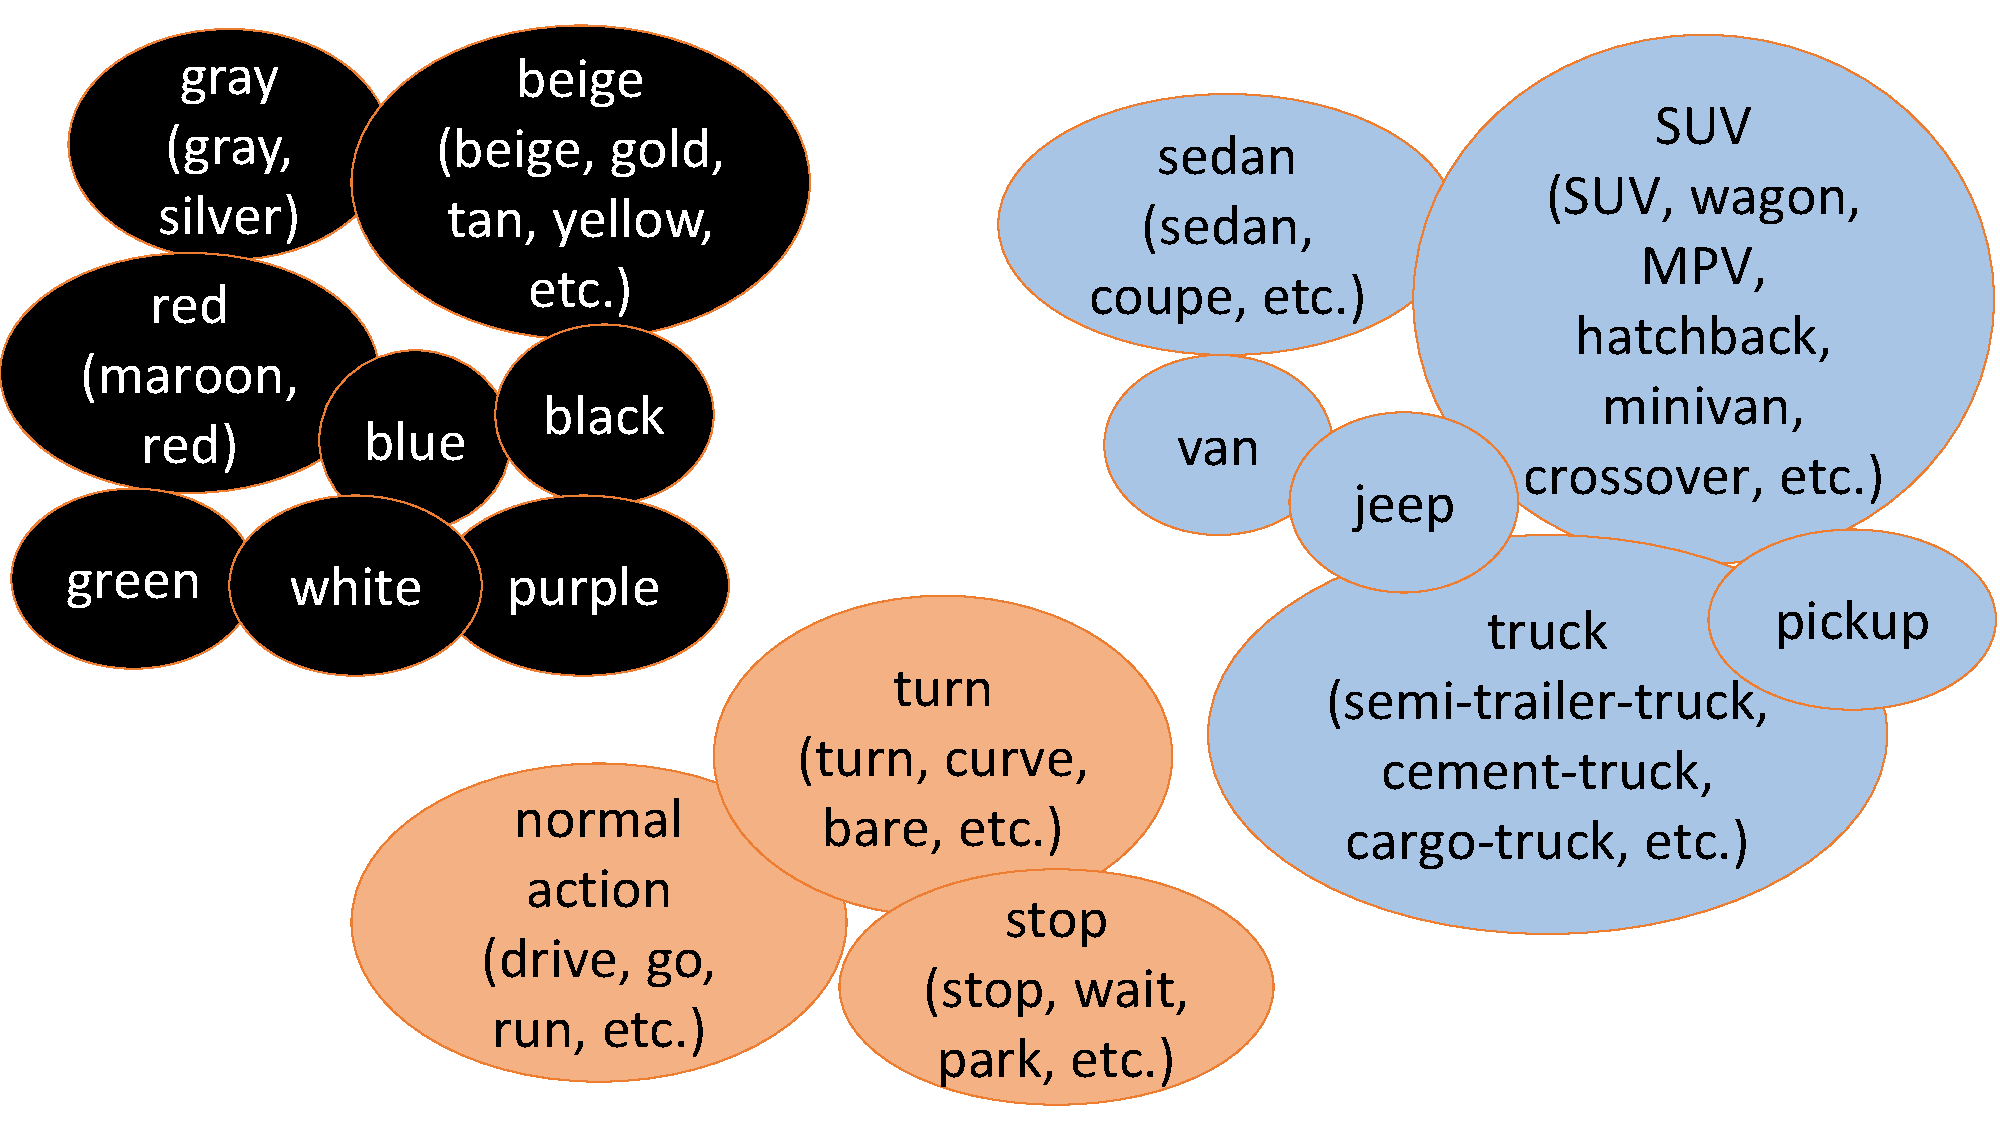
\includegraphics[width=\textwidth]{images/methods/group_example.pdf}
    \caption{How we categorize three attribute types. The black, orange, and blue shapes show the group of color, action, and vehicle type, respectively.}
    \label{fig:group_example}
\end{figure}

\begin{figure}[t!]
    \centering
    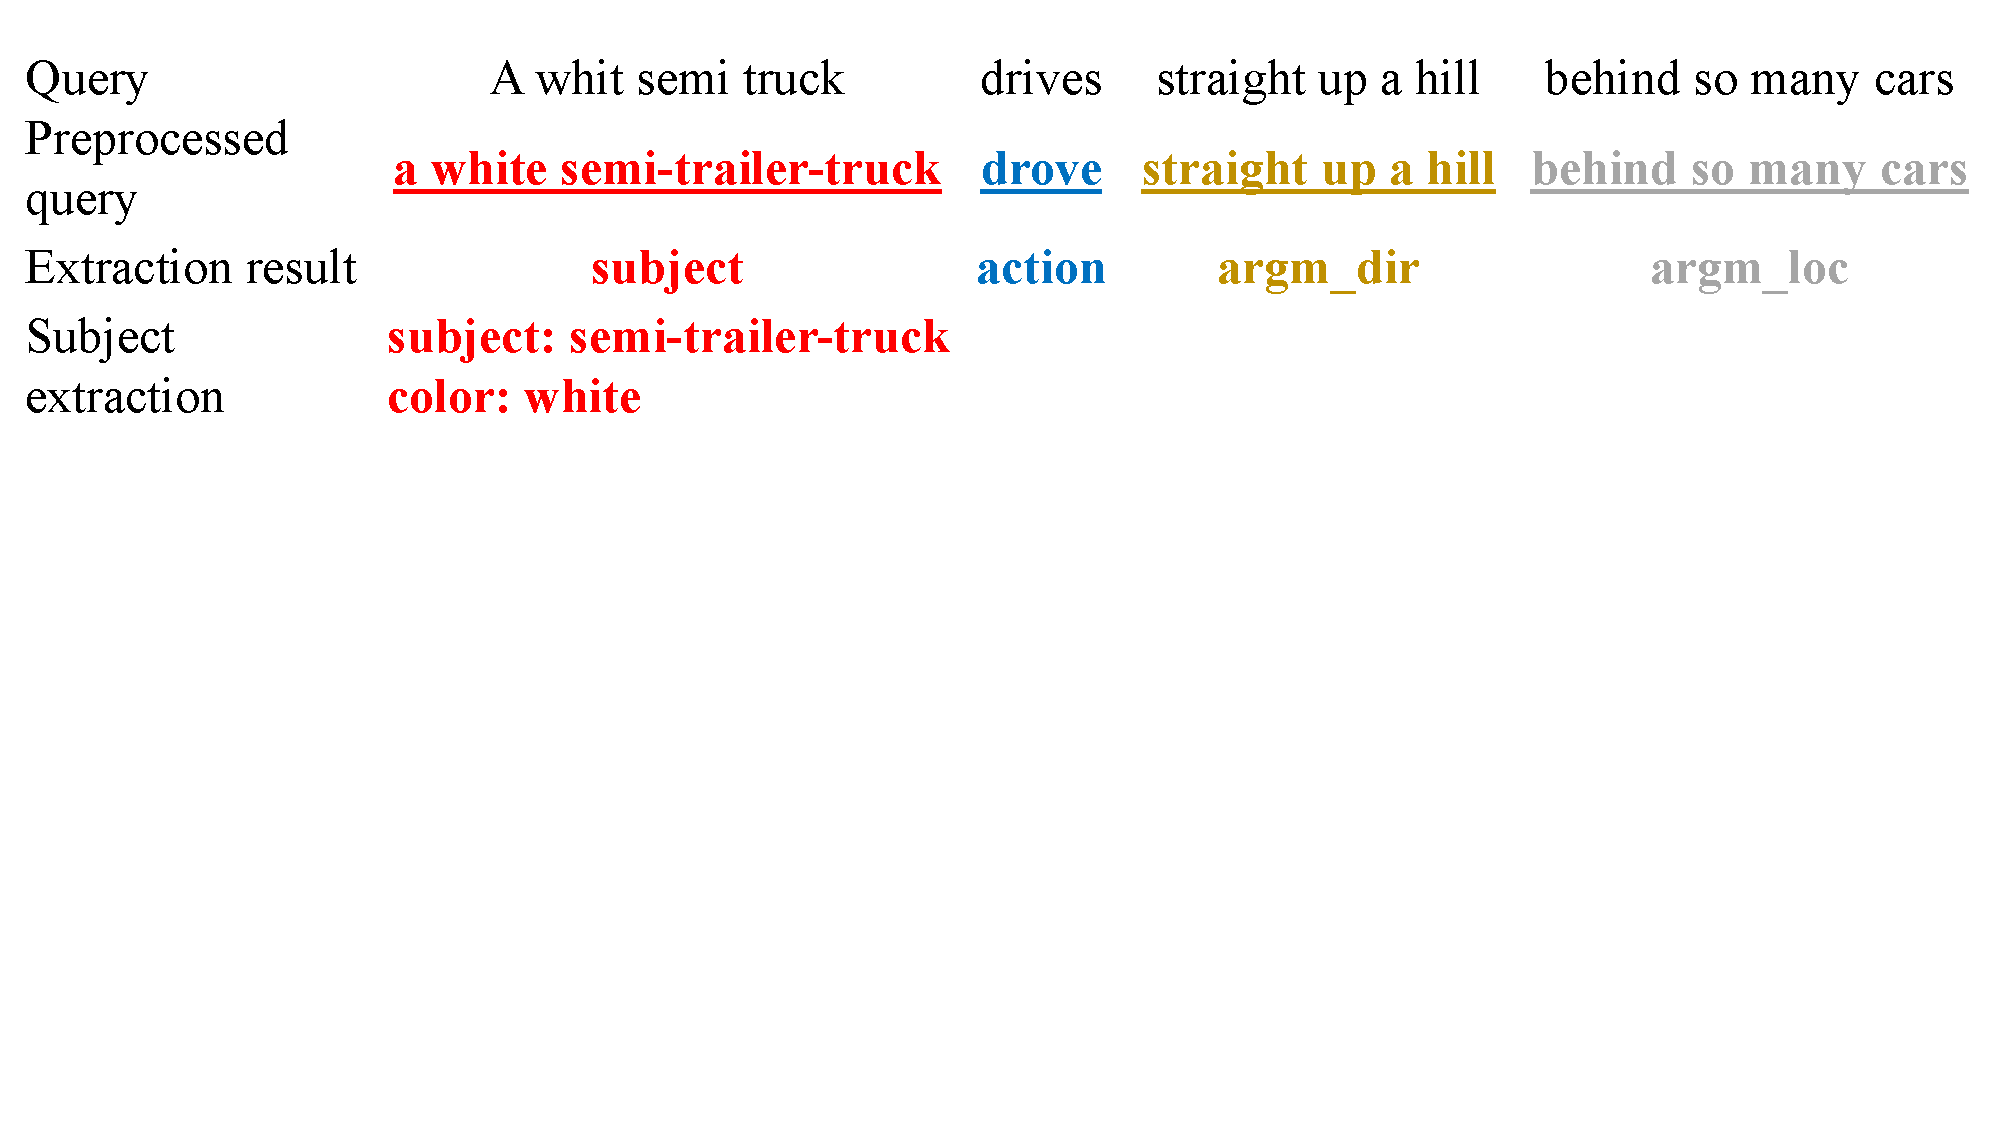
\includegraphics[width=\textwidth]{images/methods/text_extraction_example.pdf}
    \caption{An example of a query transformed and extracted through 2 stages of the heuristics method.}
    \label{fig:text_extraction_example}
\end{figure}
To make the SRL predictor work efficiently, the query needs to be corrected if it has wrong spelling. We use the Levenshtein distance metric to convert a target word to a source word in our defined vocabulary collection of vehicle attributes. To avoid the false convert, we set the condition of correcting a distance equal to 1 between the target word and the source word. We also add a rule to skip certain words which are not misspelled but have a distance of 1. For example, in the preprocessed query provided in Figure \ref{fig:text_extraction_example}, we have changed the wrong word \textit{“whit”} to \textit{“white”} but kept the word \textit{“so”} although it has the Levenshtein distance equal to 1 with the word \textit{“go”}. After this step, there is another collection containing rules to convert inconsistent words or phrases into a common one and/or verbs that are easily confused with nouns into past tense. As seen in the mentioned example, we have also made the word \textit{“semi truck”} (in the same group with \textit{“semi-truck”}, \textit{“tractor-trailer”}) become \textit{“semi-trailer-truck”}, and the word \textit{“drives”} become \textit{“drove”}. When finishing this stage, all of the essential terms related to traffic have been clear enough to be extracted.
\subsection{Extraction stage}
\begin{figure}[!htb]
    \centering
    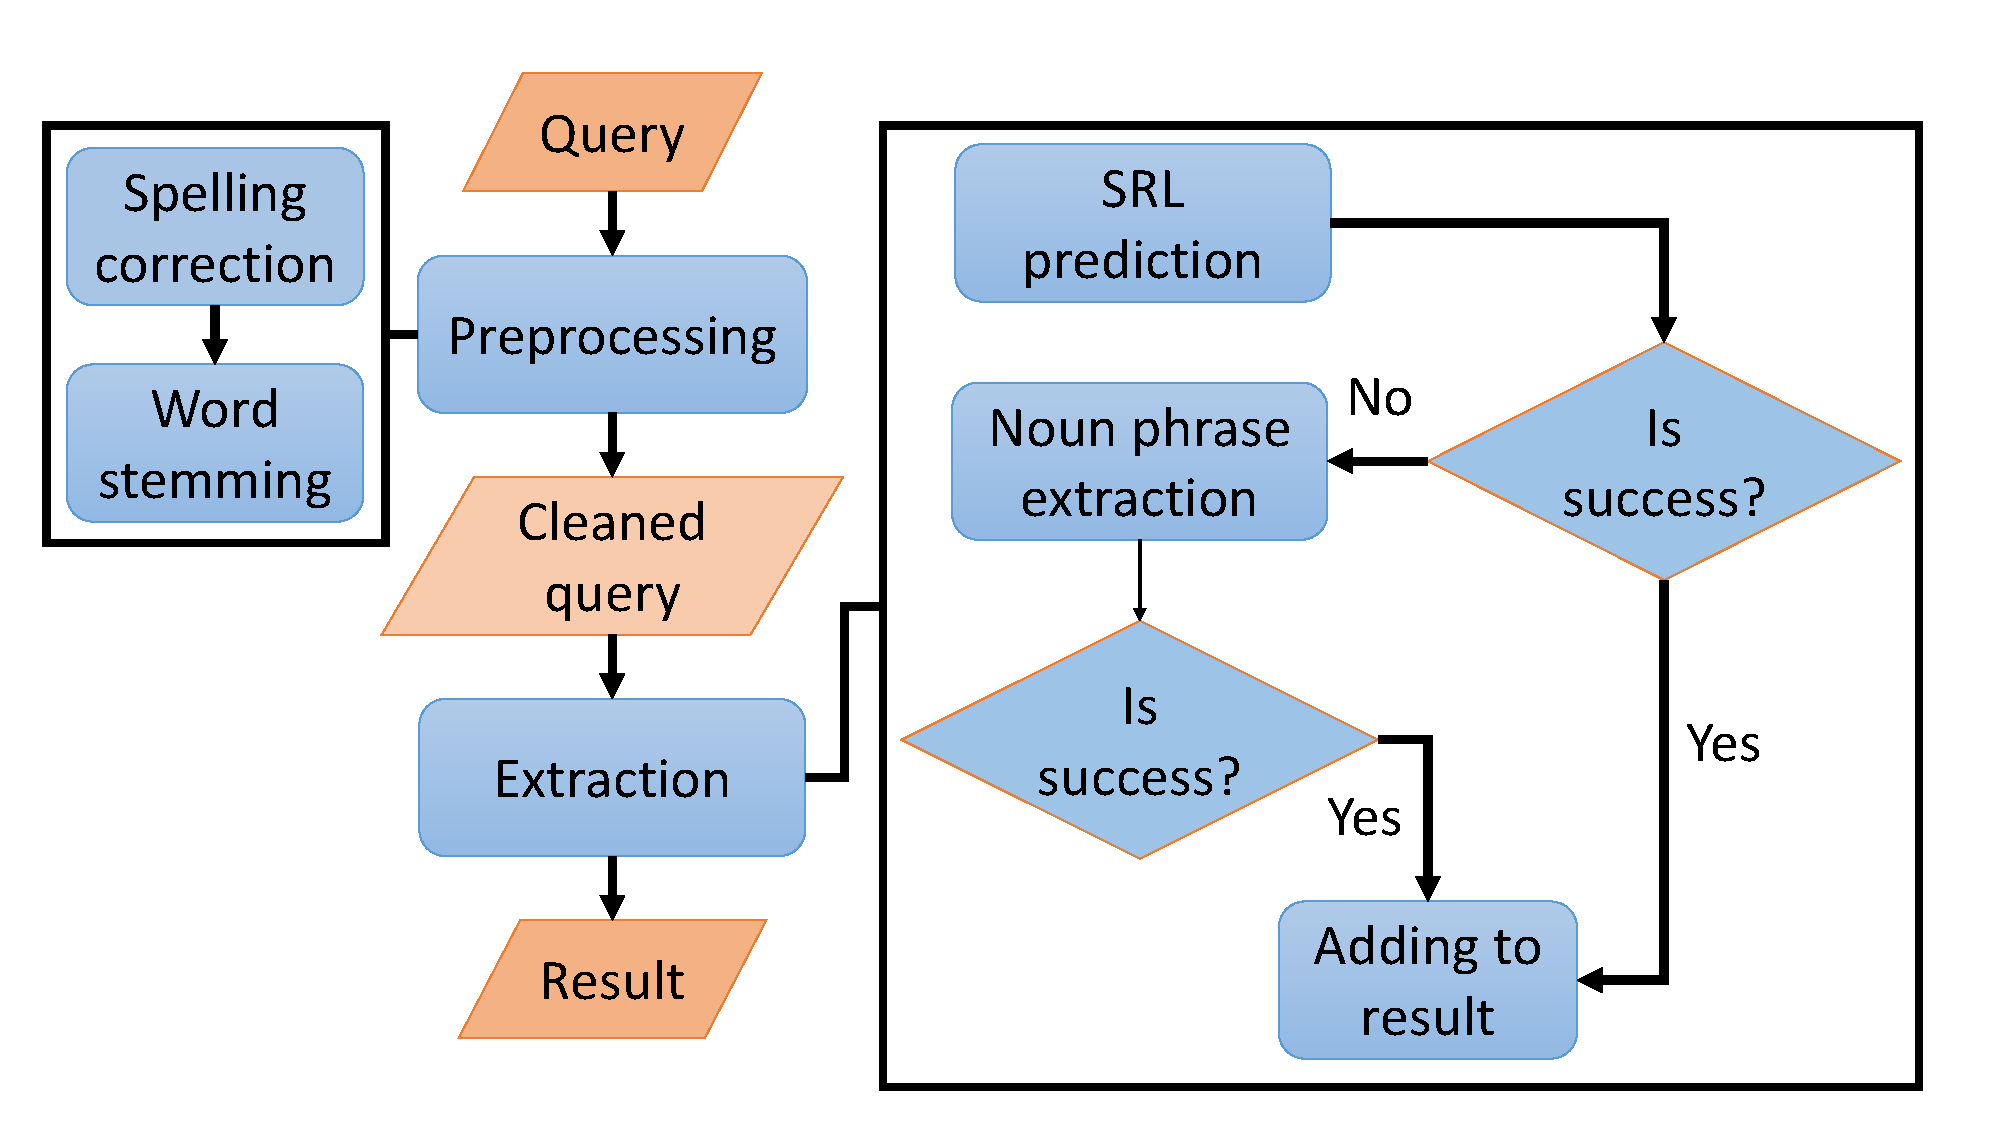
\includegraphics[width=\textwidth]{images/methods/stage_2_overview.pdf}
    \caption{An overview of the heuristic method to extract a query into SRL parts.}
    \label{fig:text_branch_stage_2_overview}
\end{figure}
For each query, a predictor toolkit is used to obtain parts of the SRL result. If the query is a complete sentence, the function will extract successfully. Otherwise, the query can be a noun phrase, and hence we must use another method to handle this. In this situation, we will collect the result if we can find the subject and confirm it as a vehicle type (i.e., \textit{a white truck}, \textit{a typical jeep}), or it will be skipped (i.e., \textit{straight on the main road}, \textit{light short to the right}).



% \section{Visual Attribute Extraction}
\label{sec:video_extraction}
\subsection{Appearance attributes extraction}
\label{sec:vehcol_extraction}
We build two modules, color encoder $E_{col}$ and vehicle encoder $E_{veh}$, with EfficientNet \cite{tan2019efficientnet} backbone to learn the visual features representation for each target vehicle from the video tracks.
The encoders are trained as a classification task, which takes the target bounding boxes as input and learns to classify them to the most reasonable groups extracted from the previous query processing step (section \ref{sec:text_extraction}). \\
\begin{figure}[!h]
    \centering
    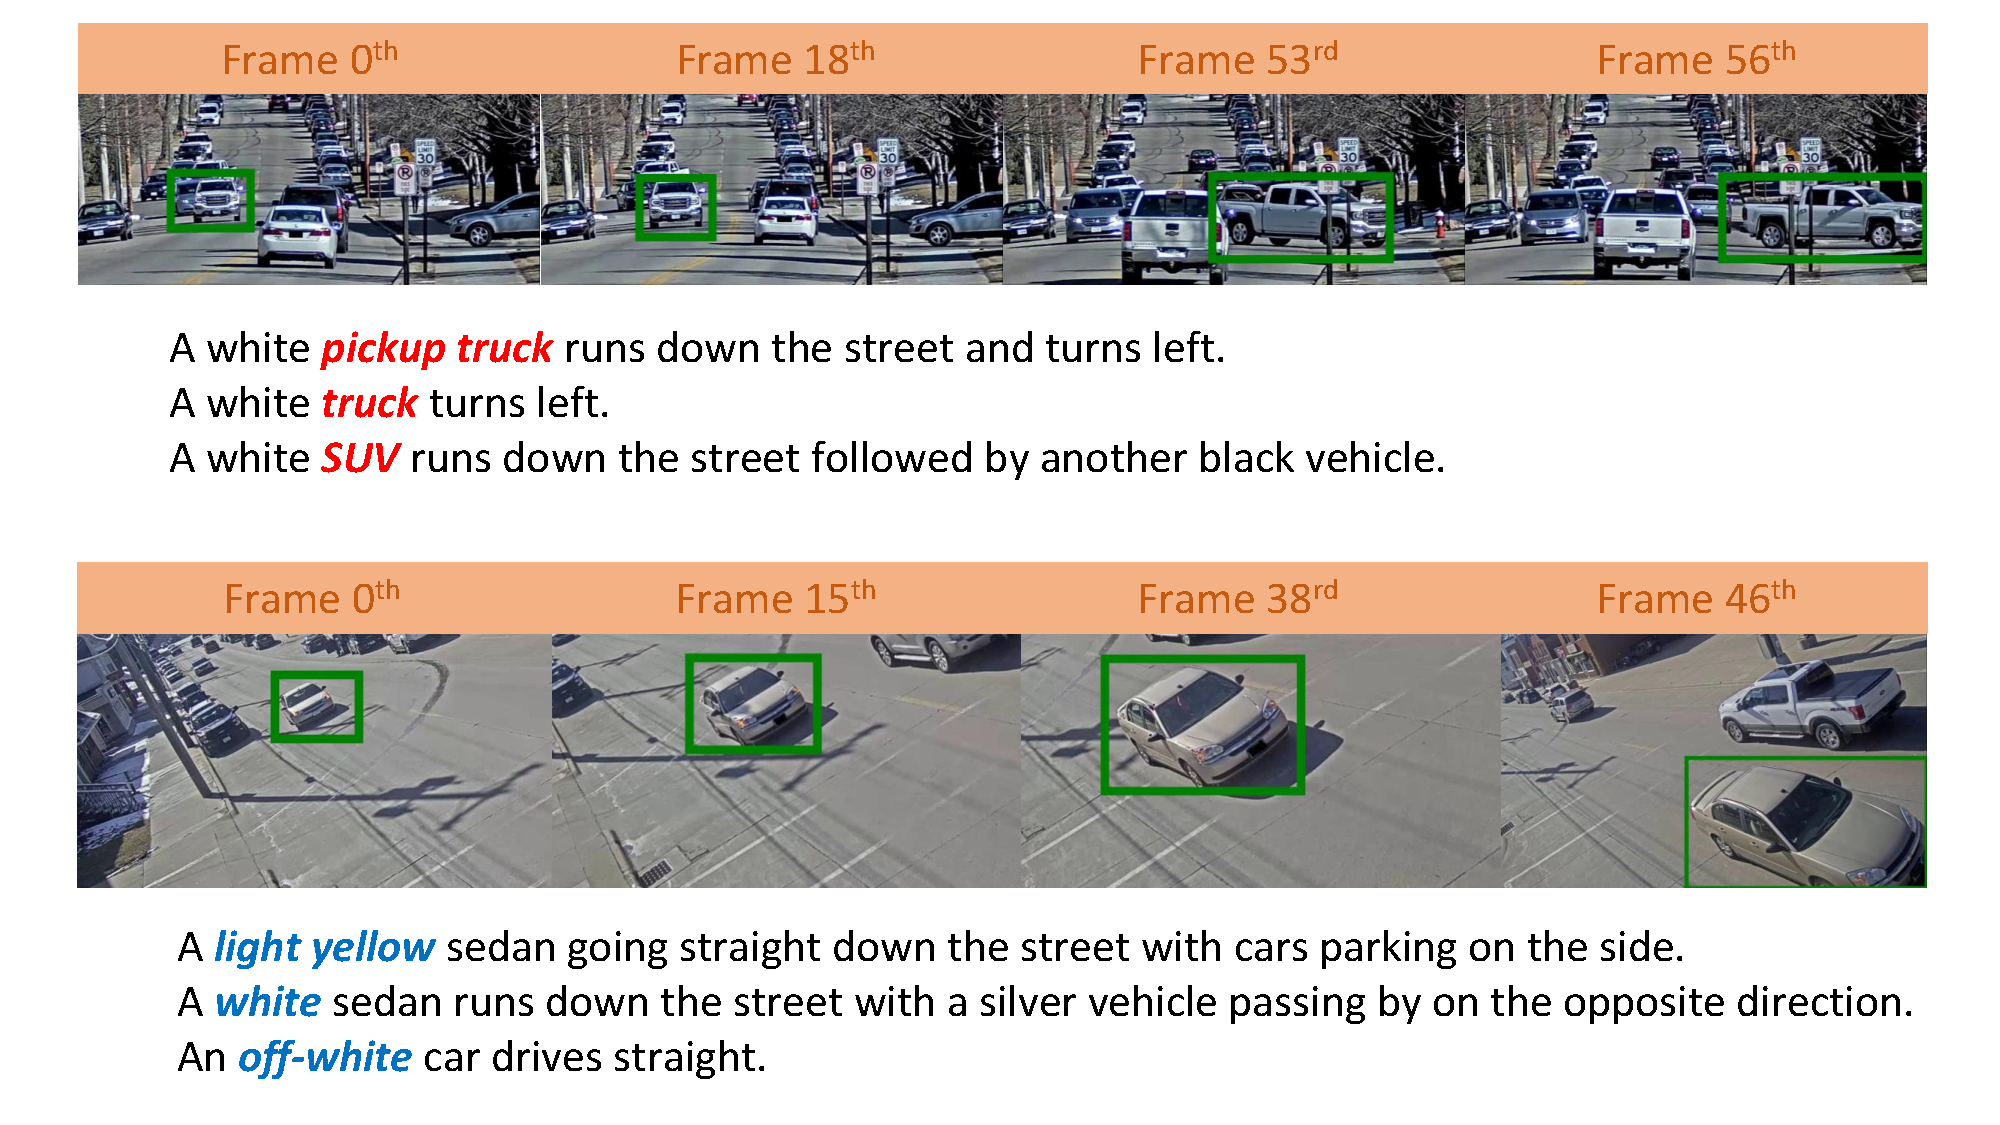
\includegraphics[width=\textwidth]{images/methods/hard_classification.pdf}
    \caption{Examples of ambiguous color/vehicle type labelling affected by different viewpoints or external influences.}
    \label{fig:hard_color}
\end{figure}
\begin{figure}[!h]
    \centering
    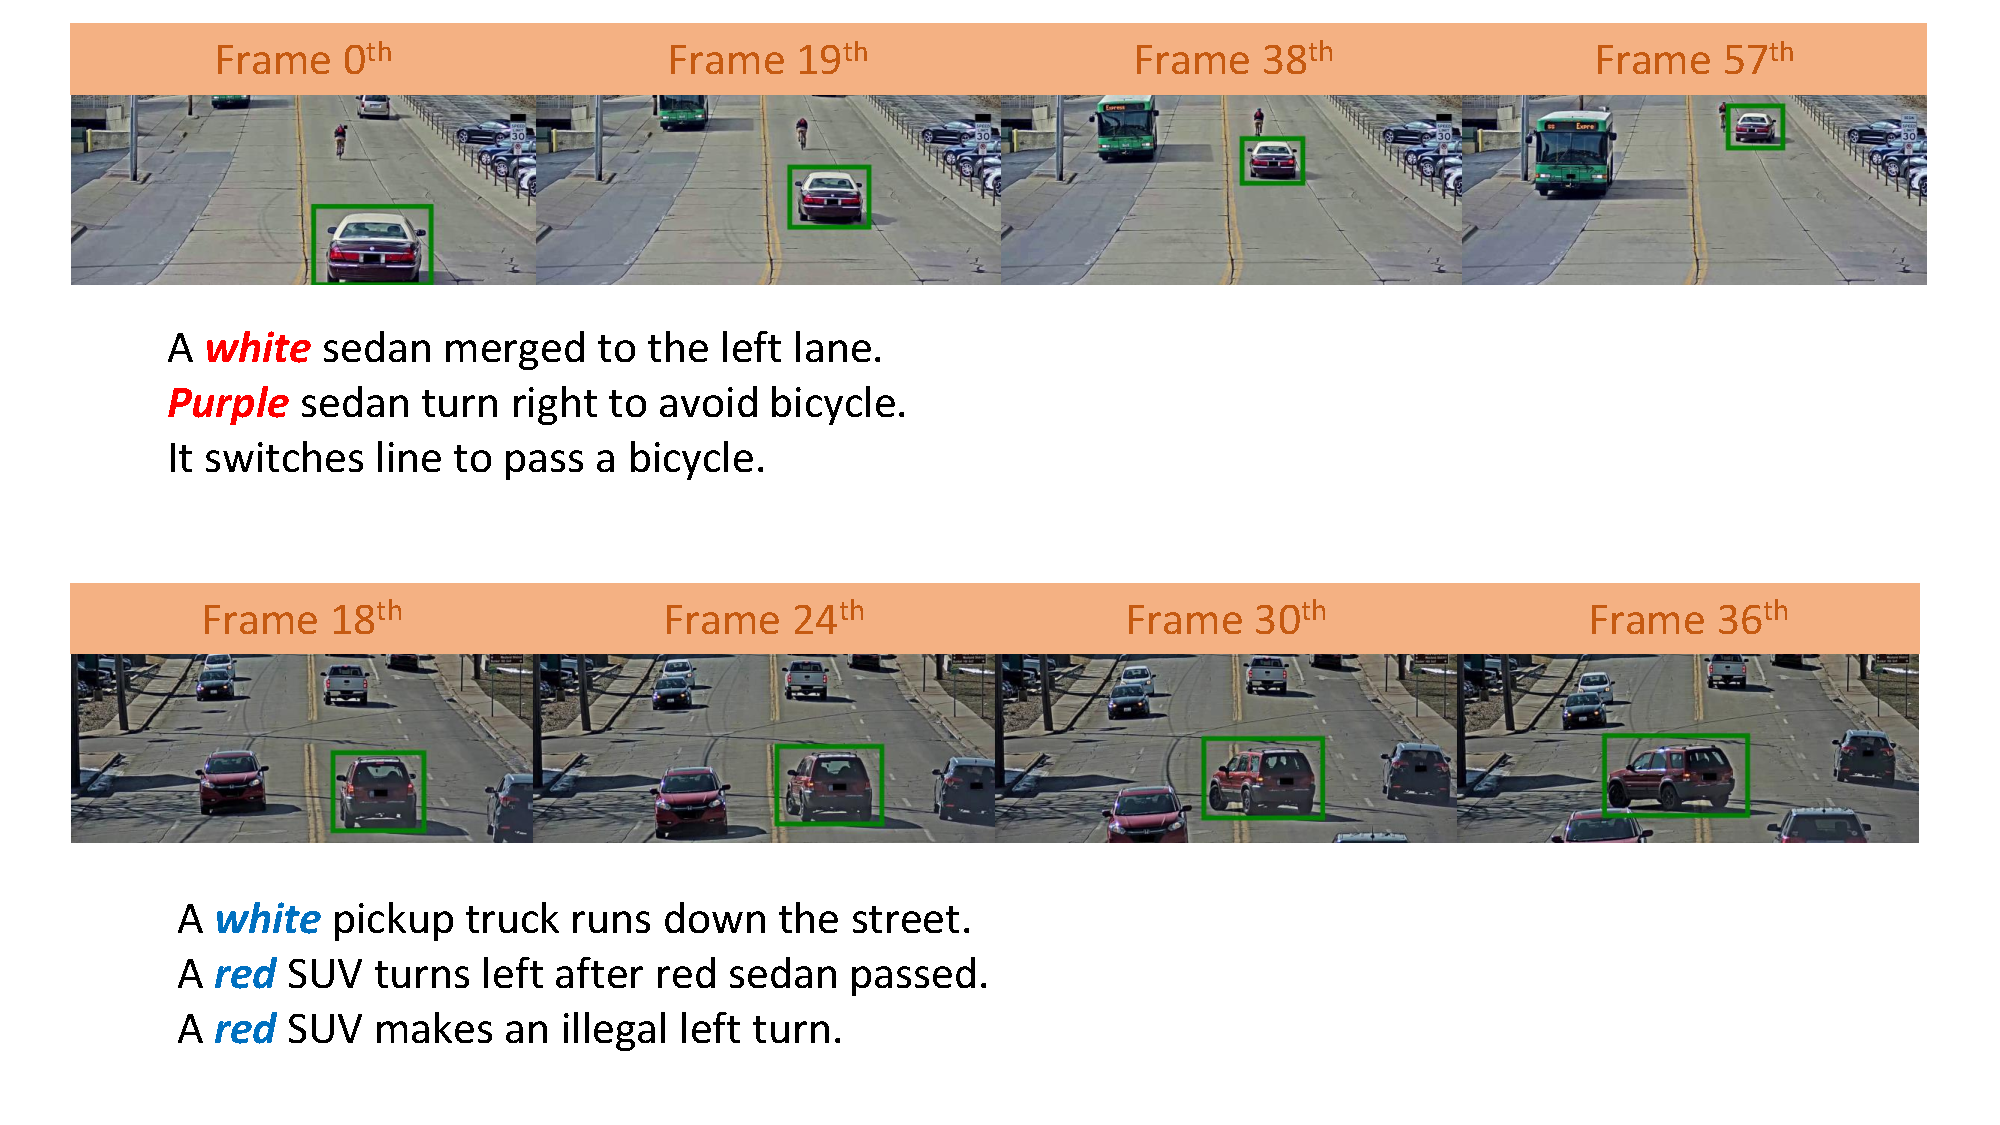
\includegraphics[width=\textwidth]{images/methods/multicolor_example.pdf}
    \caption{Examples of multi-color vehicles.}
    \label{fig:multicolor}
\end{figure}
However, in practice, the vehicle's visual attributes are not consistent between different viewpoints or could be easily affected by external conditions (sunlight, dust), as pointed in Figure \ref{fig:hard_color}. 
Also, there are some cases the vehicle itself has multi-color, as shown in Figure \ref{fig:multicolor}.
Therefore, instead of labeling each main subject with a specific class, we gather all textual attributes provided by the three captions as the multi-label ground-truth for each target. Then, we train the classifiers with multi-label approaches, where a sigmoid function replaces the softmax activation in the classification layer. \\
About the training images, for a given track with $T$ frames and $T$ temporal bounding boxes, we sample four boxes: $[B_0, B_{T/3}, B_{2T/3}, B_{T-1}]$ to handle this problem.
\subsection{Action Detection}
\label{sec:action_detection}
From the description of a query, we can obtain multiple actions of a vehicle of interest, such as \textit{``go straight''}, \textit{``stop''}, \textit{``turn right''}, \textit{``turn left''}, and so forth. In this section, we present our method to detect two important action types: stop and turn (left or right). Our method analyzes the trajectory of a vehicle, a sequence of points $p_1$, $p_2$, ..., $p_n$, where $p_i$ is the center of the vehicle's bounding box at the $i^{th}$ frame.
\subsubsection{Stop Detection}
To detect a stop event, we first calculate a sequence of motion speed $v_i$ = $dist(p_{i+k}, p_i)$ where $dist$ is the Euclidean distance and $k = 5$ in our implementation. To remove noise of a temporary slow down in speed, we apply a moving average filter with the window size $delta = 10$ on the sequence of $v_i$. We consider a stop event occurs when the speed is significant small, comparing to the average speed. We choose a simple yet efficient formula to detect a stop event if the motion speed $v_i < \alpha \times mean\{v_i\}$ where $\alpha = 0.15$.

\subsubsection{Turn Detection}
\begin{figure}[!htb]
    \centering
    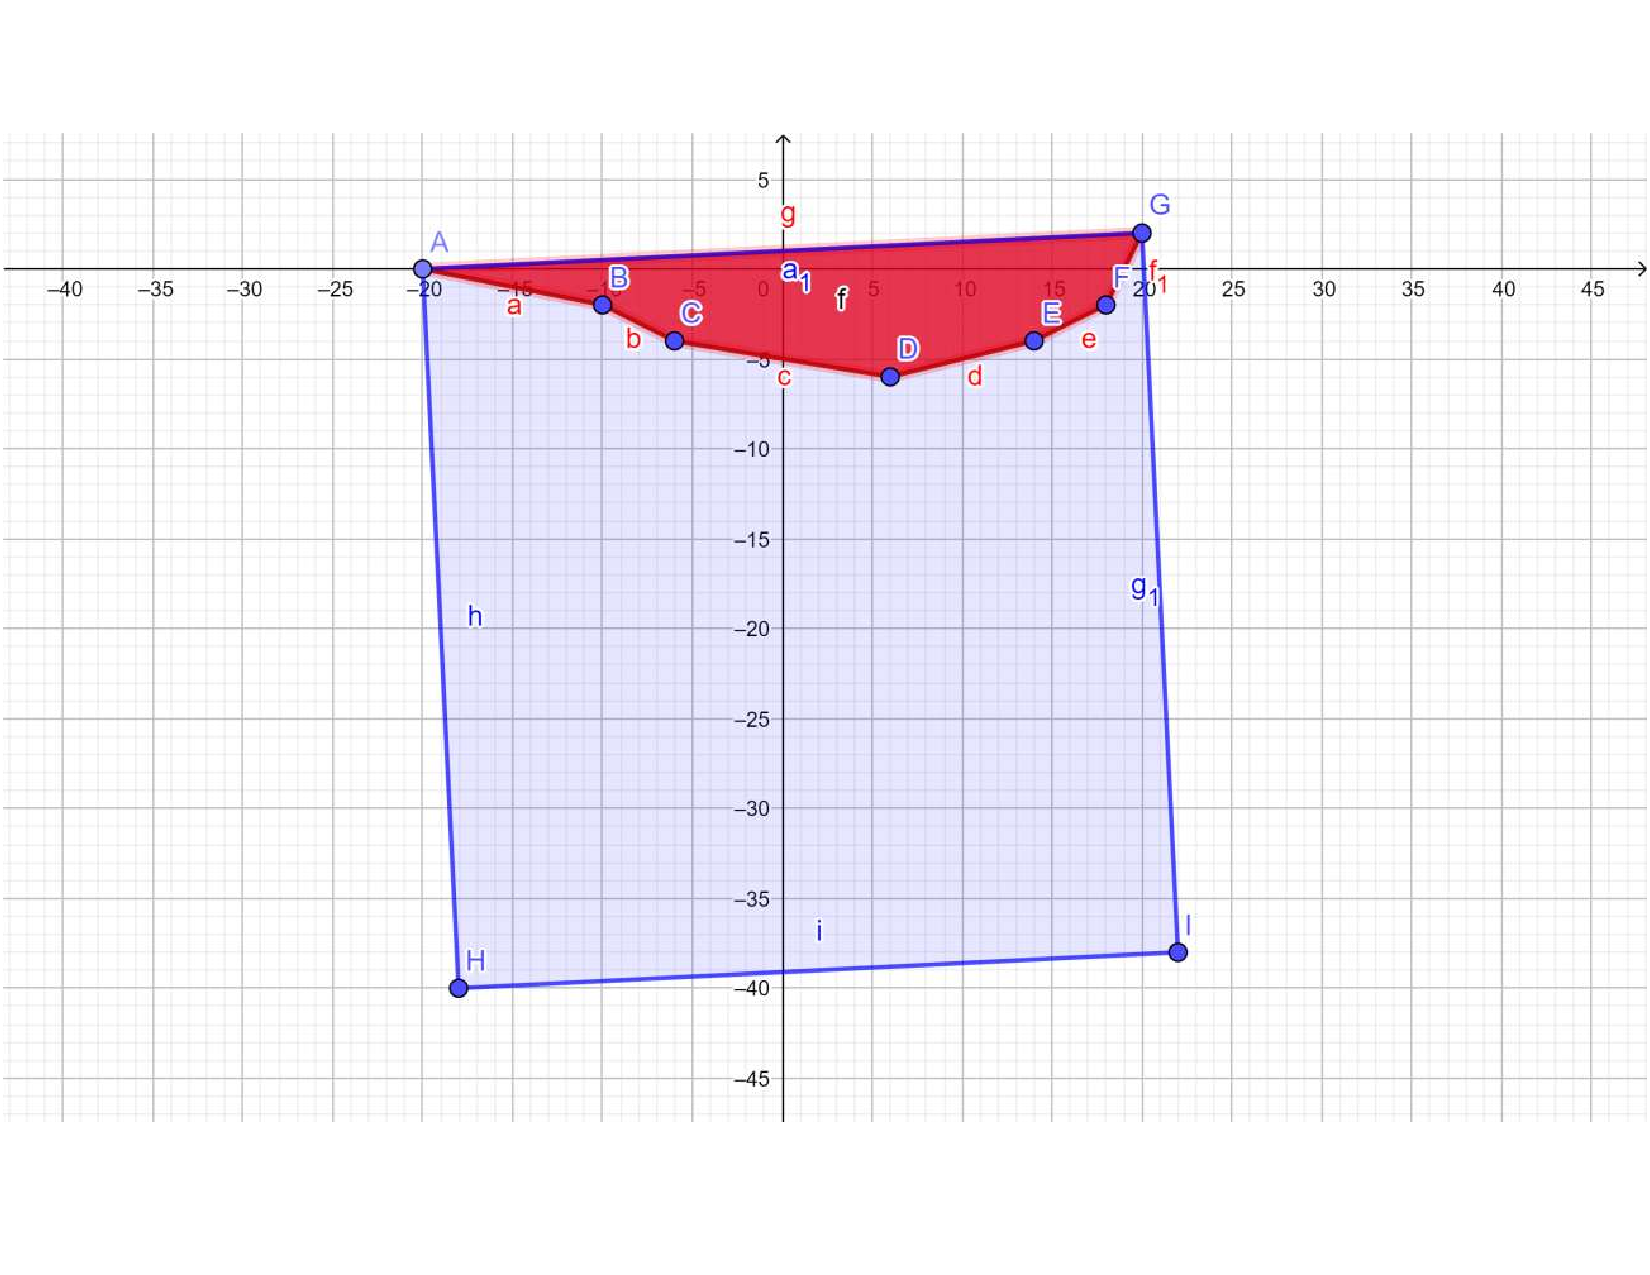
\includegraphics[width=\linewidth]{images/methods/SignedArea_foxit.pdf}
    \caption{Illustration for using algebraic area to evaluate the direction of a motion trajectory.}
    \label{fig:signed_area}
\end{figure}
We use algebraic area to classify the motion direction of a vehicle's trajectory into 3 categories:  \emph{``go straight''},  \emph{``turn right''}, and \emph{``turn left''}. 
Let $A$ be the algebraic area corresponding to the polygon with $n$ vertices $p_1$, $p_2$, ..., $p_n$. 
\[
A = \frac{{\sum\nolimits_{i = 3}^n {\overrightarrow {p_1 p_{i - 1} }  \times \overrightarrow {p_1 p_i } } }}{2}
\]

The vehicle is going in a straight line if $|A|$ is small. If $|A|$ is considerably large, the vehicle is like to turn left or right. The vehicle turns left when $A > 0$, and turns right when $A < 0$.
We observe that the error due to possible distortion in cameras is directly proportional to the square value of the distance between the start and end points in the trajectory $|p_1p_n|^2$.
We define $B = A/|p_1p_n|^2$. As illustrated in Figure \ref{fig:signed_area}, $B$ is the (signed) ratio between the area of the red polygon and the blue square. If $|B|$ is greater than a certain threshold $\epsilon$, we conclude that the vehicle turns (left or right), and goes straight otherwise.

\subsection{Relation Modeling}
\label{sec:relation_modeling}
In this section, we focus on extracting relationships between the target and those nearby vehicles. 
First we custom the DeepSort algorithm to efficiently track all vehicles attending on each video, resulting in a list of trajectories beside the provided one. Then we use these tracklets to gather all location, visual cues and perform classification prediction tasks (discussed in section ...) to achieve a detailed description of each existing vehicle including appearance attributes (vehicle type, color) and action types.
From this information, we then build a module to analyse the movement direction, relative distances between the target vehicle and all detected vehicles and determine if the target \textit{is following} them or \textit{being followed} by the others. 
Figure ... illustrates the workflow of our proposed process.

\subsubsection{Exploring surrounding objects}
Given a video track, we adapt a pre-trained object detector to localize all appearing vehicles on each frame. Then we adapt a feature extractor trained with ReID settings to obtain the appearance feature of each bounding box. The tracking algorithm then greedily compares similarity between these boxes frame-by-frame to associate all potential vehicles. Two consecutive boxes are seen as indicating the same object when their appearance similarity is lower than a pre-defined threshold. 

The AI City Challenge is launched with the intention of solving real-world problems, hence the provided training dataset contains lots of noises, which usually appear in practical scenarios. As a result, we encountered following problems when performing tracking:
\begin{itemize}
    \item High miss-frame video. In such cases, frames do not align with the correct time step. Figure … plots the distribution of miss frames in training set and test set. In some cases with extremely high miss rate (over 400 frames), the vehicles could suddenly change their positions or disappear from the video. This noise directly damages the tracking performance, especially when applying IoU distance for similarity measurement.
    \item Uncertain vehicles. From the view of traffic cameras, there are some areas where the vehicles are occluded by other obstacles (trees, traffic signs, etc.) or when the vehicles move far away from the cameras’ receptive field, they become noises for the detector.
\end{itemize}
To overcome the missed detection issue, we first generate an attention area for each video track to force the tracking algorithm to focus on those high confident detections only during the matching process. 
The attention masks are generated as follow:
\begin{itemize}
    \item Given the target vehicle tracklet, we produce a smooth trajectory by generating boxes for those missed frames with the assumption that the vehicle move linearly in the uncaptured time. For two bounding boxes $B_k$, $B_{k+1}$ corresponding to frames $F_k$ and $F_{k+1}$, the bounding boxes in between are interpolated by
    \begin{align}
        B_c = \frac{F_{k+1} - F_c}{F_{k+1} - F_k} \times B_k + \frac{F_{c} - F_k}{F_{k+1} - F_k} \times B_{k + 1}, \quad F_c \in (F_k, F_{k+1})
    \end{align}
    where $B_c$ denotes the bounding box at frame $F_c$. 
    \item Given the smooth trajectory, we enlarge the bounding box at each time step by a scale ratio $\alpha$ to create an attention mask. The final attention area of each video is the union of those masks through time.
\end{itemize}
Then, we remove those boxes that lie out of the attention area, which usually contains small vehicles, missed detections or too far vehicles. Figure ... shows a result of this step.

\subsubsection{Tracking-based relation modeling}


\pagebreak
% \section{Retrieval model}
\label{sec:retrieval_model}
\subsection{Overview}
\begin{figure}[!htb]
    \centering
    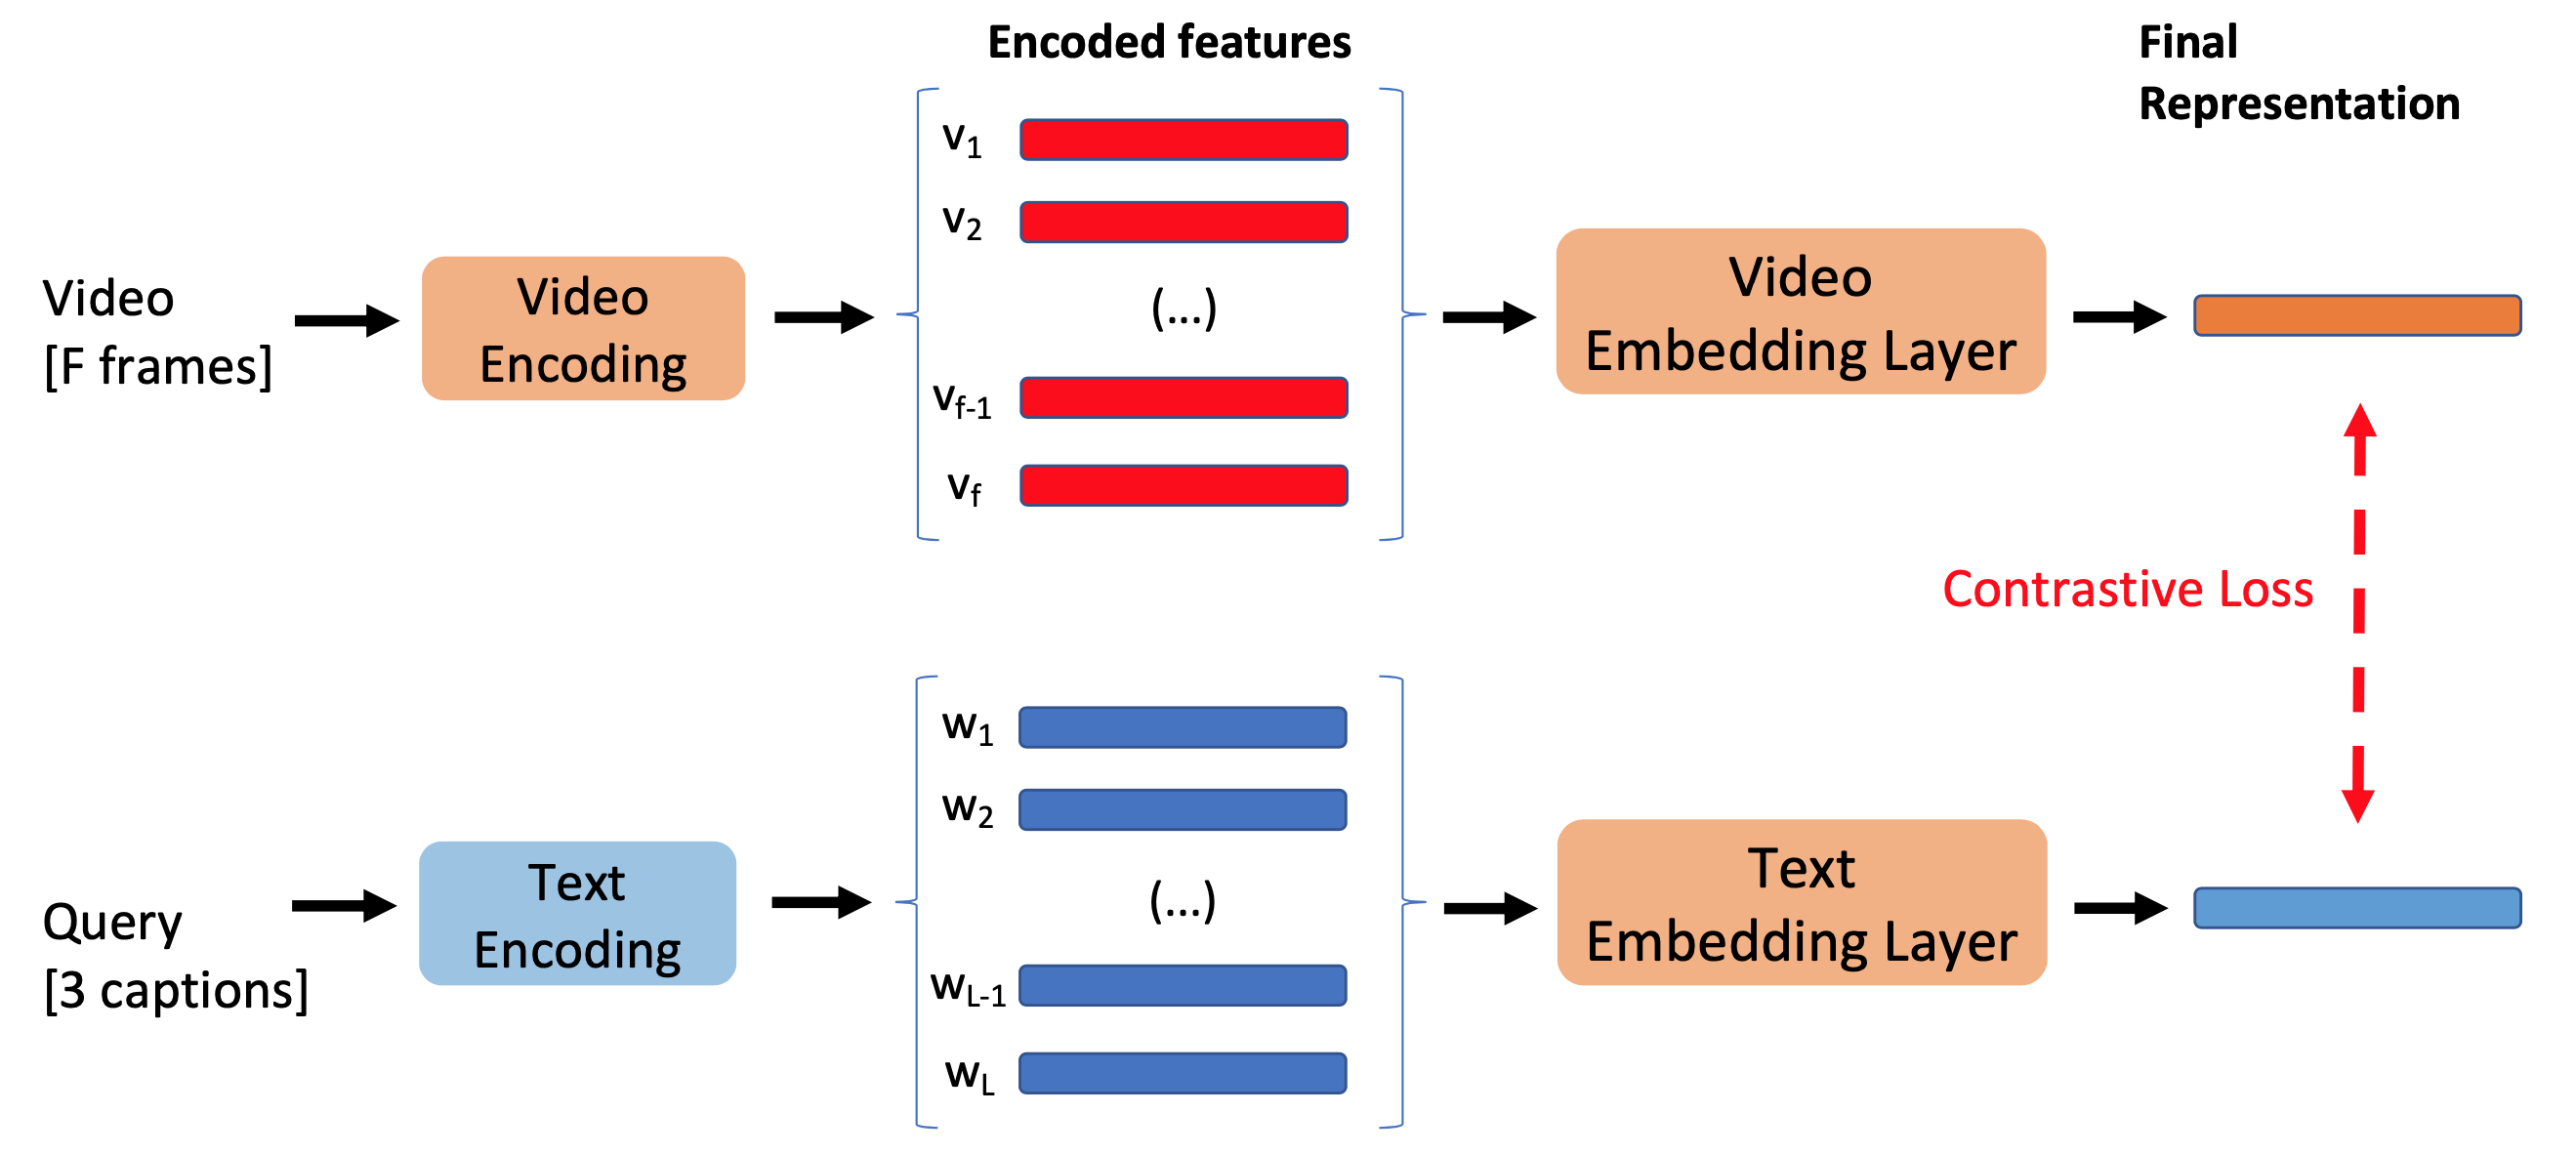
\includegraphics[width=\linewidth]{images/methods/retrieval_model.png}
    \caption{Retrieval model architecture.}
    \label{fig:ret_overview}
\end{figure}
Representation learning-based (RL-based) retrieval methods have shown potential results in various modalities. 
Especially for sequential data such as video and text, the attention mechanism provides a powerful technique for rich feature extraction, which leads to many success in cross-modalities learning tasks (as discussed in section \ref{sec:video-text_ret}). 
To efficiently apply this method to the vehicle-based retrieval problem, we employ a transformer-based architecture to learn the representation for video and text input, in which, the video encoded input is constructed from the target's essential appearance features. 
We inherit the embedding backbone of the COOT framework \cite{ging2020coot}, with some modification for better fit with our scenario.
Figure \ref{fig:ret_overview} summarizes our proposed approach.

\subsection{Representation learning}
\subsubsection{Query encoding [TODO: attribute-aware]}
In text branch, we can naively model the paragraph input in many different ways by choosing one from the combinations of three different sentences for each query.
However, we observe that the three descriptions can contain mutual meaning. For instance, the later caption may have reference to the former one.
\begin{itemize}
    \item \textit{\underline{Yellow car} keeps straight.}
    \item \textit{\underline{A yellow coupe} keeps straight before a diverging road.}
    \item \textit{There was a black pickup behind \underline{the vehicle}.}
\end{itemize}
Thus, in the encoding step, we aim to concatenate those descriptions as a whole paragraph, which provides the complete information for a specific target track.
For a query $q_i = [s_{i=1:3}]$, the preparing process is setup as follow:
\begin{enumerate}
    \item Splitting each sentence $s_i$ into a list of tokens.
    \item Encoding each token to a $d_{word}$-dimension vector. Consequently, the sentence vector is therefore a list of word vectors.
    \item Concatenating the three-sentence vectors as a final representation $\mathbf{v_{query}}$ for the query.
\end{enumerate}

\subsubsection{Video encoding}
In video branch, the video track also contains the local information of the target vehicle, which is usually the main subject and provides potential visual attributes described in the given query. For that reason, different from the original COOT method, we also include the target's attribute features in the video encoding vector. \\
In the COOT framework, given a video $V$ with $F$ frames, the video encoding is constructed by concatenating all $F$ frame-level feature $d_F$-dimension vectors, which are extracted by pretrained backbones.
For each frame, the feature vectors, enriched by deep neural networks pretrained on large benchmark datasets, contain helpful global information but lack local ones, which could be the target vehicles we need to focus on in the CityFlow-NL setup. 
From this point of view, we modify the frame-level encoded vectors with the following strategy.
Let $\mathbf{v_{frame}}$ denotes the feature vector for each frames in a video track, $\mathbf{v_{frame}} \in \mathbb{R}^{d_f}$. We define this feature as a combination of three sources:
\begin{enumerate}
    \item \textbf{Global context information ($\mathbf{v_{global}}$)}. The element aim to provide general information of each video frame.
    \item \textbf{Attributes representation ($\mathbf{v_{veh}}$)}. The compact feature produced by the attribute classifiers (section \ref{sec:vehcol_extraction}) provides the important details of the target vehicle that the model needs to focus on during the retrieval process.
    \item \textbf{Target vehicle location ($\mathbf{v_{loc}}$)}. The relative location and size of target vehicle at each time step, provide the main subject's movement trajectory information.
\end{enumerate}
For the $\mathbf{v_{global}}$, we apply the same approach as the COOT framework, which is the global feature extracted by the ResNet-152 \cite{he2016deep} pretrained on ImageNet \cite{russakovsky2015imagenet}. 
The $\mathbf{v_{veh}}$ is constructed as a concatenation of color and vehicle-type encoded vectors ($\mathbf{v_{veh-col}}$, $\mathbf{v_{veh-type}}$) provided by the corresponding encoders $E_{col}$ and $E_{veh}$, details in \ref{sec:vehcol_extraction}.
\[ 
\mathbf{v_{veh}} = concat(\mathbf{v_{veh-col}}, \mathbf{v_{veh-type}})
\]
And the vehicle location component is constructed from the bounding box coordinates at a given frame.
\[
\mathbf{v_{loc}} = [x/W, y/H, w/W, h/H]
\]
where $(x, y, w, h)$ denotes the box top-left coordinate, width, height. $(W, H)$ are respectively the width, height of the video frame. 
\begin{figure}[!h]
    \centering
    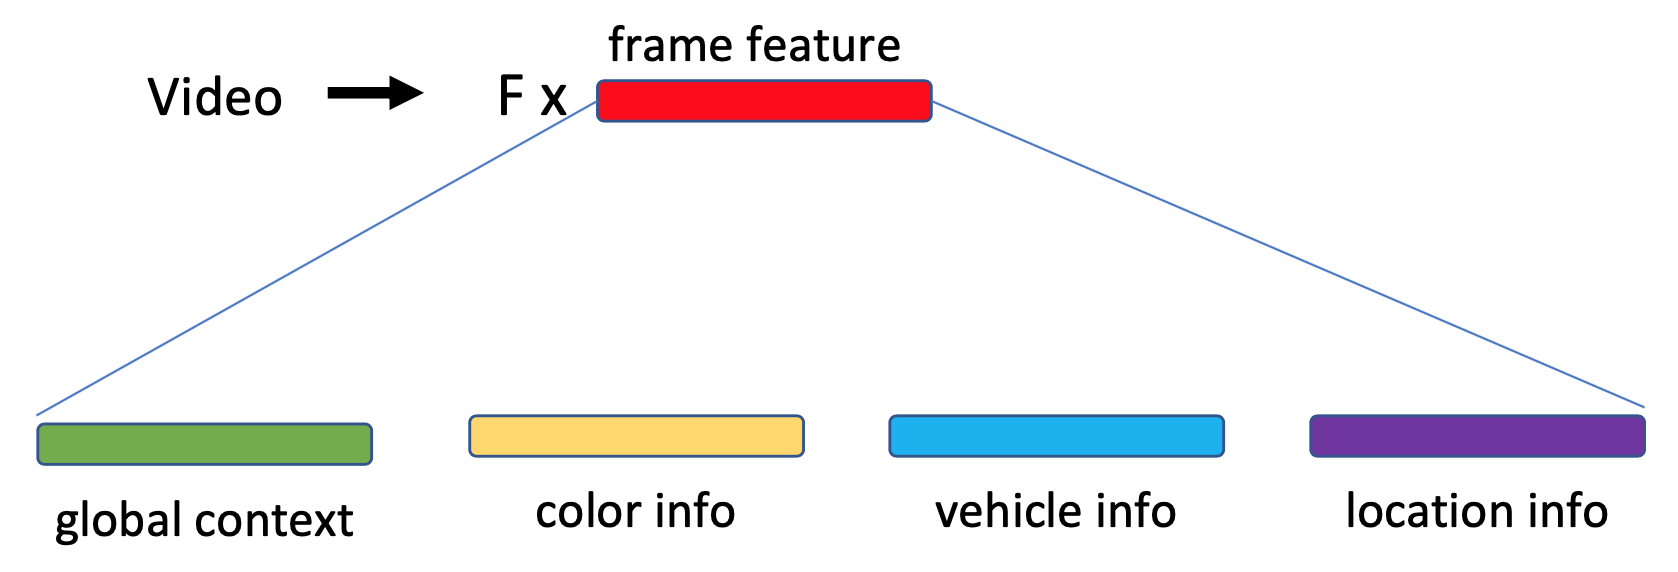
\includegraphics[width=\linewidth]{images/methods/video_encoding.png}
    \caption{Video encoding procedure.}
    \label{fig:video_encoding}
\end{figure}

In total, the frame encoded feature is modelled as:
\[
\mathbf{v_{frame}} = concat(\mathbf{v_{global}}, \mathbf{v_{veh}}, \mathbf{v_{loc}})
\]
which contains both global context and target's descriptive informations. And the final encoding for each F-length video track $\mathbf{v_{track}}$ is the combination of F frame-level features, resulting in $F \times d_f$-dimension vector (illustrated in Figure \ref{fig:video_encoding}).
The track/query representation feature ($\mathbf{v_{track}}$, $\mathbf{v_{query}}$) is then fed forward through the corresponding encoding blocks to obtain the final embedding vectors.

\subsection{Loss function}
To efficiently train the retrieval model, we inherent the alignment loss of Zhang et al. \cite{zhang2018cross}, which leverage the contrastive loss to enforce the positive samples to stay closer and the negative ones far apart. 
Given a positive sample $P = (q_i, v_i)$, set of two negative pairs $N = \{({q_i}', v_i), (q_i, {v_i}')\}$ and a margin $\alpha$, they define the following loss:
\begin{equation}
\begin{split}
    L(P, N, \alpha) = & \mathrm{max}(0, \alpha + D(q_i, v_i) - D({q_i}', v_i)) + \\ 
    & \mathrm{max}(0, \alpha + D(q_i, v_i) - D(q_i, {v_i}'))
\end{split}
\end{equation}
% \begin{align}
%     L(P, N, \alpha) = & \mathrm{max}(0, \alpha + D(q_i, v_i) - D({q_i}', v_i)) + \\ 
%     & \mathrm{max}(0, \alpha + D(q_i, v_i) - D(q_i, {v_i}'))
% \end{align}
Where $D(x, y) = 1 - \frac{x^{\top}y}{\left \| x \right \|\left \| y \right \|}$ denotes the cosine distance between two representation vectors, $q_i$ and $v_i$ indicate the embedding vectors of query and video respectively. \\
The alignment loss is defined as follow.
\begin{align}
    L_{align} = \sum_{k \in B, i, {k}'\neq k, {i}'\neq i} L((q_i, v_i), \{({q_i}', v_i),(q_i, {v_i}')\}, \beta)
\end{align}
where $B$ denotes the batch of samples at each training step, $\beta$ is the constant margin.
% \section{Relation modeling}
\label{sec:relation}
% \section{Refinement method}
\label{sec:refinement}
In the retrieval module (section \ref{sec:retrieval_model}), we have encoded the visual feature using information from color, vehicle types, and location of the target object. However, we did not exploit the motion features of the tracked objects. Therefore, we build another module to further refine the previously obtained results. In particular, this module focuses on the assessment of similar motion extracted from the query and the video track. The annotation action results of the text are retrieved from the second phase of SRL extraction (section \ref{sec:text_extraction}). Meanwhile, the annotation results of the video action are obtained from the stop and turn detector (section \ref{sec:action_detection}). The retrieval results are refined with the following priorities, i.e., motion, color, and vehicle types. The details of the refinement process are as follows:

